\chapter{XChange: A Universal Mechanism for Asset Exchange between Permissioned Blockchains}
\label{chapter:xchange}

\emph{Permissioned blockchains are increasingly being used as a solution to record transactions between companies.
Several use cases that leverage permissioned blockchains focus on the representation and management of real-world assets.
Since the amount of incompatible blockchains is quickly growing, there is an increasing need for a universal mechanism to exchange, or trade, digital assets between these isolated platforms.
There currently is no \emph{universal} mechanism for inter-blockchain asset exchange without a requirement for trusted authorities that coordinate the trade.}

\emph{In this chapter we address this shortcoming and present XChange, a universal mechanism for asset exchange between permissioned blockchains.
To achieve universality and to avoid trusted authorities that coordinate a trade, XChange does not provide atomic guarantees but leverages risk mitigation strategies to reduce value at stake.
Our mechanism records the specifications and progression of each trade within records on a distributed log.
XChange reduces the economic gains of adversaries by bounding the total amount of fraud they can commit at any time.
After having committed fraud, an adversary is forced to finish its ongoing trades before it can engage in new trades.}

\emph{We first present a four-phased protocol that coordinates an asset exchange between two traders.
We then outline how trade records can be stored on TrustChain, which is a lightweight distributed ledger specifically built for the tamper-proof storage of data elements.
We implement XChange and conduct experiments.
Our experiments demonstrate that XChange is capable of reducing the economic gains of adversaries by more than 99.9\% when replaying a real-world trading dataset.
A deployment on low-resource devices reveals that the latency added to a trade by XChange is only 493 milliseconds.
Finally, our scalability evaluation shows that XChange achieves over 1'000 trades per second and that its throughput, in terms of trades per second, scales linearly with the system load.}

\newpage

\section{Introduction}
Bitcoin, introduced in 2008, has revolutionized the field of digital currencies by demonstrating that it is possible to devise a secure cash system without a bank~\cite{nakamoto2008bitcoin}.
The goal of Bitcoin is to realize a payment system through the secure management of a native currency on a distributed ledger.
The creation of this currency is controlled by miners participating in a voluntary process known as mining.
The collective efforts of miners ensure the security of Bitcoin and prevent illegitimate coin creation.
Miners invest computational power to include valid transactions on the blockchain, which is a tamper-proof distributed ledger that consists of blocks.
One of the compelling features of a blockchain is the ability to securely record and validate user-issued transactions without trusted authorities, even in the presence of mutual distrust between participants.

Participation in many deployed blockchains is open for everyone and does not require the explicit approval from authorities unlike traditional banking systems.
Even though blockchain technology provides the means to maintain a distributed ledger without trusted authorities, open enrollment is not required for many industrial use cases, or is even undesirable.
For instance, when two companies leverage blockchain technology to securely record their transactions, read and write access to the distributed ledger is most likely limited to a few selected employees or operators.
Over the past few years, there has been a sharp increase in the development and deployment of private, or \emph{permissioned} blockchains~\cite{androulaki2018hyperledger,de2018pbft,vukolic2017rethinking}.
In contrast to a public blockchain like Bitcoin, membership in a permissioned blockchain is managed by an authority that approves the participation of each peer.
The identity under which a peer operates is linked to a real-world persona, which reduces the likelihood of Byzantine behaviour and network threats like the Sybil Attack~\cite{douceur2002sybil}.
Permissioned blockchains usually adopt a classical consensus model designed for networks with static membership, e.g., Practical Byzantine Fault Tolerance (PBFT)~\cite{castro1999practical}.
Considerable efforts in permissioned blockchains have been made by projects such as Hyperledger Fabric~\cite{androulaki2018hyperledger}, R3 Corda~\cite{brown2016introducing}, Quorum~\cite{mogan2018quorum} and BigchainDB~\cite{mcconaghy2016bigchaindb}.
Permissioned blockchains have the potential to increase the efficiency of traditional business processes in industries like logistics, energy management and trade supply chains~\cite{vukolic2017rethinking}.

Several use cases that record transactions on a permissioned blockchain revolve around the representation and management of real-world assets on a distributed ledger~\cite{hewett2019inclusive}.
Advancements in blockchain technology have resulted in numerous platforms on which companies can issue and manage digital assets.
There currently is a proliferation of different types of assets, fragmented across many different blockchain implementations~\cite{borkowski2018towards}.
In public blockchains, almost 200'000 different assets are being managed on the Ethereum blockchain only.\footnote{See \url{https://etherscan.io/tokens}}
A recent Forbes report reveals that at least 50 major companies, each valued at least at \$1 billion, are exploring blockchain technology for asset management and trading~\cite{forbes50companies}.
As industry's adoption of blockchain technology is increasing, a similar asset proliferation will occur with permissioned blockchains.
Unfortunately, there is no \emph{universal} mechanism to exchange (trade) assets between isolated distributed ledgers without the involvement of a trusted third party.
Research and developments in distributed ledger technology mostly focus on the deployment of new domain-specific blockchains, whereas interoperability issues are mostly ignored~\cite{schulte2019towards,yli2016current}.
In particular, there is a lack of research on the interoperability of permissioned, industry-grade blockchains~\cite{nikander2019interledger,vo2018internet}.
Interoperability concerns are particularly relevant when leveraging distributed ledgers for trading, as a single trade consignment can involve various isolated blockchains~\cite{ganne2018can}.
Given the inevitable growth of permissioned blockchain platforms, we argue that a universal mechanism for asset exchange between these platforms is a growing necessity.

\begin{figure}[t]
	\centering
	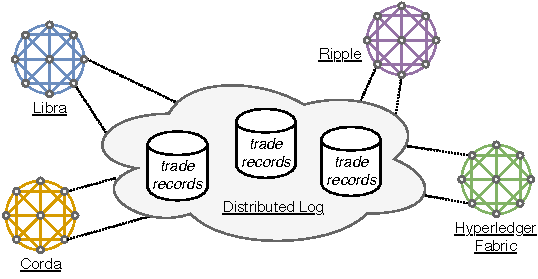
\includegraphics[width=.8\linewidth]{xchange/assets/xchange_interoperability}
	\caption{\ModelName{} coordinates the asset exchange between permissioned blockchains by storing trade records in a distributed log. This enables traders to detect if a party has committed fraud during an ongoing trade.}
	\label{fig:xchange_interoperability}
\end{figure}

We present \emph{\ModelName{}}, a universal mechanism for asset exchange, or \emph{trade}, between permissioned blockchains.\footnote{We use the terms \enquote{exchange} and \enquote{trade} interchangeably in this work.}
\ModelName{} coordinates trade between separate permissioned blockchains by storing trade records in a distributed log, also see Figure~\ref{fig:xchange_interoperability}.
Our solution is independent of the technical characteristics of the involved blockchains and does not require modifications to blockchain applications that are already operational.
An asset exchange in \ModelName{} proceeds through a sequence of alternating, unilateral asset transfer operations (payments) between two parties.
This is comparable to how many electronic markets (e.g., eBay) operate, where a party only initiates a payment back to the counterparty after having received a payment first.
Sequential payments, however, introduce a risk of losing economic value to the other party, since the other party is now able to \enquote{steal} assets during a trade~\cite{koens2019assessing}.
This fraud is called \emph{counterparty fraud} and it is a severe concern in many electronic marketplaces that facilitate peer-to-peer trading~\cite{peters2016understanding}.
For this reason, we argue that any asset trading mechanism must either prevent counterparty fraud or punish a participant that has committed this fraud upon its detection.

To address counterparty fraud, blockchain-based asset exchange often provides \emph{atomic} guarantees.
Atomicity in this context implies that a trade either exchanges all assets between involved parties or exchanges nothing.
We find that the security of existing trade solutions either (1) relies on (semi-trusted) authorities to ensure that assets are securely exchanged, or (2) relies on the availability of specialized transactions by the blockchains that manage the assets being traded.
Relying on authorities is the standard approach when trading assets managed by public blockchains, e.g., by using the services of a cryptocurrency exchange.
In a permissioned setting, however, this approach requires the participation of these intermediaries in the involved blockchains, which is not always allowed by their network operators.
Asset exchange mechanisms that depend on specialized transactions, e.g., atomic swaps~\cite{nolan2016atomic}, are not universal enough to support asset exchange between any pair of permissioned blockchains.

In contrast to existing solutions, \ModelName{} particularly focuses on the \emph{detection} of counterparty fraud.
We argue that the detection of counterparty fraud during a trade is sufficient, since misbehaviour can always be traced back to a real-world identity, and optionally be punished by an external authority.
To detect counterparty fraud, \ModelName{} requires traders to append tamper-proof trade records to a distributed log.
By recording the initiation of each trade, conducted payments, and the completion of a trade, participants can detect if a malicious trader has committed fraud and then refrain from trading with that party.

\ModelName{} does not provide atomic trade guarantees; however, it bounds the economic gains of adversarial parties by introducing two risk mitigation strategies.
First, \ModelName{} allows a trade to gradually complete through multiple, smaller payments.
We refer to this technique as \emph{incremental settlement}.
With incremental settlement, traders themselves decide how much risk they are willing to take, and specify how much economic value they put at stake.
Our second risk mitigation strategy is to bound the value that traders are entrusted with during ongoing trades.
This bound is decided by traders themselves and enables a trader to still be engaged in multiple lower-risk trades.
\ModelName{} forces an adversarial party to finish its ongoing trades first before it can engage in other high-valued trades.
We prove that this approach bounds the economic gains of adversaries.
Since \ModelName{} assumes static membership through well-defined identities, it prevents a situation where a participant that has committed counterparty fraud can re-joins the network under a new digital identity and commit fraud again (the whitewashing attack~\cite{feldman2006free}).

In this work, we first present and classify existing mechanisms for cross-blockchain asset exchange.
We then outline our solution and describe the \ModelName{} protocol.
We deploy \ModelName{} using a tamper-proof, distributed log with low overhead, a technology that pre-dates Bitcoin~\cite{haeberlen2007peerreview}.
Specifically, we leverage an existing solution, TrustChain, that is built for the secure logging and accounting of generic data elements~\cite{otte2017trustchain}.
Our experiments with real-world trading data reveal that our risk mitigation strategies can reduce fraud gains by 99.9\%.
By conducting a trade between two Raspberry Pis, we quantify that the added latency by \ModelName{} is only 493 milliseconds.
Additional experiments on our compute cluster reveal that \ModelName{} can handle over 1'000 trades per second and that its throughput scales linearly with the system load.

%The fundamental design principle of \ModelName{} is to \emph{decouple trade management and the exchange of assets between traders}.
%The key design principle of \ModelName{} is to \emph{decouple order management and asset management}.
%Our approach is visualized in Figure~\ref{fig:idea} and originates from the observation that existing blockchain-based marketplaces for asset trading utilize the same underlying data structure to manage trade and to exchange assets.\todo{remove/rewrite?}
%Therefore, trade management is subject to the same security requirements as the exchange of assets between trading parties.
%By decoupling these two practices, we increase overall market throughput, since trade management requires different (lower) security guarantees than the exchange of assets.
%Peers in the \ModelName{} network maintain a distributed ledger that stores all orders and trade activity.
%These peers interact with external platforms to transfer assets to other traders.
%To store market activity , we build on a scalable blockchain ledger that is optimised for data accounting.
%By accounting full trade specifications, we show that the effectiveness of fraud conducted by adversarial parties is limited.

The main contribution of this work is five-fold:
\begin{enumerate}
	\item We present the \ModelName{} \emph{trading protocol} which specifies how assets are exchanged between permissioned blockchains by storing trade records in a distributed log (Section~\ref{sec:protocol}).
	\item We devise two \emph{risk mitigation strategies} that lower the risk for traders and bound the economic gains of adversaries committing counterparty fraud.
	\item We improve TrustChain, a tamper-proof, distributed log used by \ModelName{}. Our improvements enables concurrent transactions and increase scalability (Section~\ref{sec:blockchain_accounting}).
	\item We provide a functional, open source \emph{implementation} of the \ModelName{} trading protocol (Section \ref{sec:implementation}).
	\item We present \emph{experimentation} around the security, resource usage and scalability of \ModelName{}, conducted on multiple low-resource devices and our compute cluster (Section~\ref{sec:xchange_fraud_experiment} -- \ref{subsec:scalability_experiment}).
\end{enumerate}

\section{Related Work and Problem Description}
\label{sec:background_problem_description}
Achieving interoperability between blockchains is a challenging problem and remains largely unsolved~\cite{zamyatin2019sok,vo2018internet,buterin2016chain}.
Most research in this direction considers cross-chain interactions between permissionless blockchains~\cite{koens2019assessing}.
There is only few research on how to achieve interoperability between permissioned blockchains, even though this is also a concern in private environments.
We first discuss existing solutions that address asset exchange between different blockchains, ranging from approaches that rely on a central authority to trust-less trading mechanisms using specialized transactions or intermediate blockchains.
Based on our findings, we then formulate the requirements for our asset exchange mechanism.

\subsection{Central Authorities}
A common approach to exchange blockchain-based assets is by using the services of a central authority.
A trade using a central authority completes as follows: two parties that agree on a trade transfer the assets for sale to one of the wallets owned by the authority.
When this intermediary has received both assets, it finishes the exchange by transferring the appropriate assets to the other party.
In this approach, the authority holds (temporary) ownership of the assets to be traded.
Relying on a central authority removes counterparty risk for the trading parties, but it requires both parties to have faith that the intermediary does not default or compromise their assets.

Trade through a central authority can facilitate value exchange between an extensive range of different blockchains, as long as the intermediary maintains wallets on the involved blockchains and can issue transactions in these systems to transfer the assets.
This is usually not an issue in permissionless blockchains since anyone can create accounts or wallets by generating a new cryptographic key pair.
Centralized cryptocurrency exchanges often facilitate asset trading across numerous permissionless blockchains.
Some cryptocurrency exchanges process transactions worth millions of dollars in total daily.\footnote{See \url{https://coinmarketcap.com/rankings/exchanges}}
In a permissioned blockchain environment, however, a central authority coordinating an asset exchange requires explicit approval from the operator to read and write transactions on the involved distributed ledgers.
Allowing new parties in a permissioned blockchain might be undesirable by operators since it introduces additional legal and operational risks.

There have been various efforts to mitigate the trust issues surrounding centralized exchanges and trusted authorities while still maintaining a centralized infrastructure.
TEX is a centralized exchange that uses an off-chain settlement solution for trust-less asset trade~\cite{khalil2019tex}.
TEX is resilient against the front-running attack where insider information is exploited to gain a financial advantage while trading.
Tesseract leverages trusted hardware, e.g., Intel SGX, to build a secure cryptocurrency exchange that also addresses the front-running attack~\cite{bentov2019tesseract}.
The Arwen trading protocol is another protocol to securely trade cryptocurrencies through a centralized exchange without giving up ownership of the assets to the exchange~\cite{heilman2020arwen}.


\begin{figure}[t]
	\centering
	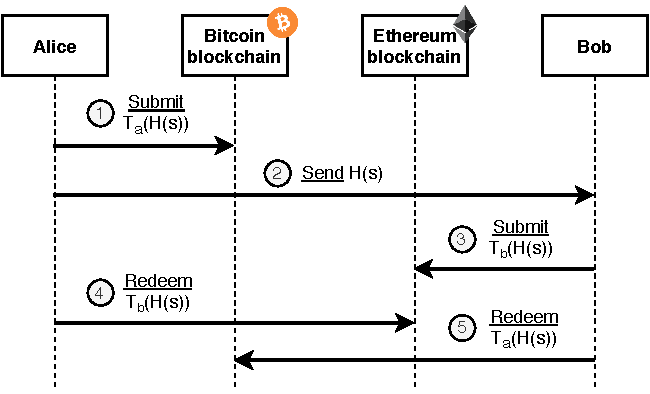
\includegraphics[width=.7\linewidth]{xchange/assets/atomic_swap}
	\caption{Sequence diagram of a successful HTLC-based atomic swap between Alice and Bob.}
	\label{fig:atomic_swap}
\end{figure}

\subsection{Atomic Swaps}
The \emph{atomic swap} is a protocol that is commonly used to exchange assets between different blockchains, without need for a central authority~\cite{herlihy2018atomic}.
Atomic swaps enable two parties to exchange blockchain-based assets in an atomic manner: the asset exchange either completes or fails for both parties at any given time.\footnote{We remark that the atomicity of the atomic swap protocol depends on the security of the underlying blockchains. If one of the blockchains is compromised by adversaries, atomicity during asset exchange cannot be guaranteed and one of the parties can lose its funds to the counterparty.}
Atomic swaps eliminate the risk of losing assets to an adversarial trader during the exchange.
The main idea is that trading users lock their assets in a specialized transaction on the blockchain in such a way that no single party can claim both locked assets.
This is achieved with \emph{Hash-Timelock Contracts} (HTLCs), a special transaction that leverages hash locks and time locks.
A hash lock is a restriction that prevents the transfer of assets until the pre-image of a provided hash is revealed.
A time lock is a primitive that locks assets until a specific time.
They prevent the assets being traded from being locked up indefinitely during an atomic swap.
This time lock should be well above the block confirmation time of the underlying blockchain to prevent the loss of assets during a blockchain reorganization.
In practice, the duration of the time lock is often fixed to several hours.

We further explain the atomic swap by considering a trade with Bitcoin and Ether (the native token of the Ethereum blockchain).
Figure~\ref{fig:atomic_swap} visualizes an atomic swap between two parties, Alice and Bob, where Alice sells her Bitcoin in return for Ether.
The basic atomic swap, described by Tier Nolan~\cite{nolan2016atomic}, consists of the following six steps:

\textbf{Step 1.} Alice generates a secret value $ s $ and computes $ H(s) $, where $ H(\cdot) $ is a secure hash function.

\textbf{Step 2.} Alice submits a hash-timelock transaction $ T_1 $ to the Bitcoin blockchain, locking her Bitcoin and using $ H(s) $ for the hash lock. A party can claim the Bitcoin held by $ T_1 $ with another transaction that provides $ s $, within a specific time duration.

\textbf{Step 3.} Alice sends $ H(s) $ to Bob using any communication medium.

\textbf{Step 4.} Bob submits a hash-timelock transaction $ T_2 $ to the Ethereum blockchain, locking his Bitcoin and also using $ H(s) $ for the hash lock.

\textbf{Step 5.} Alice claims the Bobs' Ether locked in $ T_2 $ by submitting a transaction, $ T_3 $, to the Ethereum blockchain, containing $ s $. $ T_3 $ unlocks the hash-lock in $ T_2 $. This reveals pre-image $ s $ to Bob.

\textbf{Step 6.} Bob now claims Alice's Bitcoin locked in $ T_1 $ by submitting a transaction, $ T_4 $, to the Bitcoin blockchain, containing $ s $. The asset exchange is now complete.

The above protocol requires a total of four transactions.
Note how Alice is not able to claim her assets without providing the opportunity for Bob to claim his assets.

Atomic swaps enable asset exchange between a wide range of blockchains.
Even though they are an interesting proposition for cross-chain asset trade, we describe three deficiencies of this technique.
First, atomic swaps can only be used when trading assets between distributed ledgers with support for specific programming constructs, such as time-locked and hash-locked transactions.
Both blockchains are also required to support the same hashing algorithm.
Second, atomic swaps require traders to lock their assets using a hash-timelock transaction.
This enables a Denial-of-Service attack where a party can intentionally retain the assets of a counterparty, denying the counterparty from using the locked assets for other purposes.
Third, atomic swaps can be unfair for one of the parties since the swap initiator has a time window after both parties have locked their assets, during which it can decide to abort the swap~\cite{han2019optionality}.
This window enables price speculation by the swap initiator by keeping the assets of the other party locked until the asset price goes in the favor of the initiator.

\subsection{Notary Schemes}
\label{sec:notary_schemes}
Notary schemes are another solution for asset exchange where the approval by a group of credible nodes (notaries) is required to perform some operation.
Notary schemes aim to partially alleviate the trust issues arising when relying on a central authority through the approval by a group of semi-trusted notaries instead.
These notaries reach consensus on the occurrence of particular events, e.g., on the inclusion of a transaction on a distributed ledger.
Compared to an asset exchange through a central authority, notary schemes assume a weaker trust model and can often withstand adversarial behaviour of a fraction of the notaries.

AgentChain is an asset exchange system that is based on multi-signature schemes~\cite{li2019agentchain}.
Each user can act as a trading operator, which together form trading groups.
Assets are locked in a multi-signature wallet that requires a multi-signature to unlock.
Users can choose to trade within a specific trading group, e.g., based on the reputation of the trading group.
If a trading group acts malicious, a user can upload evidence to the blockchain upon which all assets managed by that trading group are transferred back to users.

An earlier version of the Interledger protocol, ILPv1, used intermediate notaries (also called \emph{connectors}) to conduct payments across different ledgers~\cite{thomas2015protocol}.
These payments are realized through conditional payments and are coordinated by a different group of connectors for every involved ledger.
Interledger uses payment paths where additional intermediate platforms and their connectors are used to exchange assets between ledgers that do not have a direct connection.
Only when a particular condition is met, the payment is conducted.

%We argue that notary schemes work well when exchanging assets between permissioned blockchains.
%Specifically, the entities that are managing the permissioned blockchain are suitable to take on the role as notary so no involvement of new parties is required.

\subsection{Blockchain Bridges}
Another approach to cross-chain trade uses bridging techniques, where an intermediate blockchain mediates asset exchange between different blockchains.
Most bridging approaches execute the atomic swap protocol for the exchange process of assets but provide additional primitives and interoperability features for communication between blockchains.

Blocknet is a platform for inter-blockchain routing and facilitates the exchange of cryptocurrencies between blockchains~\cite{culwick2019blocknet}.
Blocknet consists of two main components: XBridge and XRouter.
XBridge is a decentralized protocol that coordinates atomic swaps between permissioned and permissionless blockchains.
XRouter provides a peer-to-peer overlay network consisting of clients running the SPV protocol, therefore avoiding the need to download the full blockchain to verify the inclusion of particular transactions.
Blocknet secures its transactions through a Proof-of-Stake consensus protocol.
Furthermore, Blocknet provides a decentralized exchange where traders can indicate their trade interests through orders.
A blockchain connected to Blocknet requires the implementation of time-locked transactions.

ARK is a platform for cross-chain asset exchange that shares similarities with Blocknet~\cite{ark2019whitepaper}.
ARK enables users to build custom blockchains (a \enquote{BridgeChain}) that is powered by the ARK blockchain.
To facilitate asset exchange between different blockchains, ARK acts as an intermediate blockchain in the trade process.
The latter is achieved through the smart bridge protocol, relying on atomic swaps to exchange value across chains.
The ARK blockchain achieves transaction security through a Delegated Proof-of-Stake (dPos) consensus algorithm, where stakeholders vote for a small committee that appends blocks to the ARK blockchain.

The Proof-of-Authority (POA) blockchain is an Ethereum-based permissioned blockchain that provides several tools for interoperability~\cite{poa2018whitepaper}.
The POA blockchain is secured by the Proof-of-Authority consensus mechanism, where validating nodes stake their reputation to secure the blockchain.
The TokenBridge protocol enables users to not only exchanges assets between Ethereum-based platforms, but also facilitates arbitrary data transfer.

\subsection{Sidechains}
Sidechains provide the means to exchange assets between blockchains that share similarities, e.g., that run a particular consensus algorithm~\cite{singh2020sidechain,back2014enabling}.
In essence, a sidechain is a blockchain that is attached to a parent chain.
With a two-way pegged sidechain, assets residing on the parent chain can securely be moved to the sidechain and vice versa.
These transfers lock the assets on one chain and re-create them on the connected sidechain or parent chain.
A related scheme is federated pegged sidechains~\cite{dilley2016strong}.
In a federated pegged sidechains, assets moving to another chain are controlled by a group of notaries, making this approach comparable to notary-based solutions (see Section~\ref{sec:notary_schemes}).
Liquid is a deployed sidechain to the Bitcoin blockchain and can be used to quickly trade Bitcoin-derived currencies~\cite{dilley2016strong}.

\subsection{Internet-of-Blockchains}
We now describe two solutions that aim to devise an \enquote{Internet-of-Blockchains}, where a single blockchain controls many sub-chains.
The Cosmos project, introduced by the Interchain Foundation, builds a network of heterogeneous blockchains that can seamlessly interact with each other~\cite{cosmoswhitepaper}.
The Cosmos Hub is the leading blockchain that connects many other blockchains, called zones.
Each zone can have its own governance rules and is secured using the Tendermint BFT consensus protocol.
Tokens can quickly be exchanged between the Hub and zones using the Inter-Blockchain Communication (IBC) protocol.
To interact with blockchains external to Cosmos, there is a particular zone, called a \emph{bridging zone}.
The bridging zone keeps track of transactions and blocks persisted on external blockchains, e.g., Ethereum.

The system architecture of Polkadot, introduced by Gavin Wood, is similar to Cosmos~\cite{wood2016polkadot}.
Polkadot introduces a single relay chain that is responsible for the coordination of one or more parachains.
Polkadot secures its chains through a custom consensus algorithm, inspired by Tendermint~\cite{kwon2014tendermint} and HoneyBadger~\cite{miller2016honey}.
Compared to Cosmos, Polkadot aims for a more generic message-passing algorithm between parachains that can not only transfer value.

Both Cosmos and Polkadot can facilitate the effortless exchange of assets between zones or parachains.
However, they have limited capabilities for interaction with external blockchains.
To benefit from the advantages that Cosmos and Polkadot provide, all involved companies must fully commit to the same blockchain platform, which is hard to achieve in practice.
Therefore, the advantage of Internet-of-Blockchains is questionable for industrial use cases, and a less demanding approach might be preferred when trading assets.

\begin{figure}[t]
	\centering
	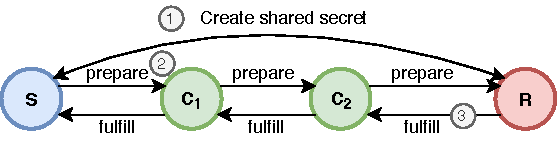
\includegraphics[width=.65\linewidth]{xchange/assets/interledger}
	\caption{A successful ILPv4 payment from a sender $ S $ to a receiver $ R $, using two connectors $ C_1 $ and $ C_2 $.}
	\label{fig:interledger}
\end{figure}


\subsection{The Interledger Protocol V4 (ILPv4)}
The Interledger Protocol V4 (ILPv4) is a protocol for conducting payments between different ledgers~\cite{ilpv4}.
Although the protocol primarily resolves around one-way asset transfers, it can also be used to exchange assets between different ledgers.
ILPv4 maintains a peer-to-peer payment network consisting of different connectors that can transfer value across heterogeneous networks within ILP packets.
In comparison to ILPv1 (discussed in Section~\ref{sec:notary_schemes}), ILPv4 is designed around the fast transfer of low-valued payments.
ILPv4 drops the requirement for ledger-based payments since they can be slow to complete and can lead to capital retention, similar to atomic swaps.
A sender and a connector are assumed to have funds on some shared network, e.g., they can maintain a unidirectional or bidirectional payment channel if an appropriate blockchain is used.

An ILPv4 payment between a sender $ S $ and a receiver $ R $ using two connectors proceeds as visualized in Figure~\ref{fig:interledger}.
First, $ S $ and $ R $ create a shared secret, which will act as the condition for the payment (step \circled{1}).
Then, $ S $ will prepare a \texttt{prepare} packet that contains the details of the upcoming payment and the details of the agreed-upon condition (step \circled{2}).
This packet is sent to an available connector, which forwards the packet to subsequent connectors until the packet reaches the receiver $ R $.
When receiving the \texttt{prepare} packet, $ R $ determines the validity of the payment as stipulated by a higher-level protocol and can either reject the payment by sending a \texttt{reject} packet back, or accept the payment by responding with a \texttt{fulfill} packet (step \circled{3}).
The \texttt{fulfill} packet contains the pre-image of the agreed-upon condition.
Connectors forwarding a \texttt{fulfill} packet verify the included pre-image against the payment condition in the previously received \texttt{prepare} packet.

The Hyperledger Quilt project provides a Java implementation of the Interledger protocol for permissioned blockchains~\cite{hyperledgerquilt}.
The project provides a set of rules for enabling ledger interoperability, formats for network packets and a framework for designing applications that leverage ILPv4.

\subsection{Information Exchange}
We end with a brief discussion on techniques for the exchange of private information across different ledger implementations.
Whereas asset exchange involves transfer of ownership, information exchange requires that the buyer does not learn the information without the seller receiving something in return.
An information exchange is said to be \emph{fair} when this aforementioned property holds~\cite{asokan1997optimistic}.

The FairSwap protocol is the most advanced approach in this direction and ensures a fair exchange of digital goods by leveraging smart contracts and arithmetic circuits~\cite{dziembowski2018fairswap}.
The protocol introduces a \emph{proof-of-misbehaviour} that proves if a seller misbehaves during an exchange.
This proof is computationally cheap to construct.
The OptiSwap protocol extends FairSwap by incorporating an interactive dispute resolution protocol, reducing the communication overhead of FairSwap~\cite{eckey2020optiswap}.
Delgrado et al., describe a protocol for fair data exchange based on the Bitcoin scripting language~\cite{delgado2020fair}.
The protocol is based on a new primitive, private key-locked transactions, that allow the atomic exchange of a private key for Bitcoin.
This private key is then used to decrypt the traded information.

\begin{table}[t]
	\centering
	\footnotesize
	\begin{threeparttable}
		\begin{tabular}{ c c c c c c } 
			\hline
			\textbf{Approach} & \textbf{Universal?} & \textbf{Avoids trusted parties?} & \textbf{Guarantees atomic exchange?} \\
			Central Authorities & \greencheck & \redcross & \redcross \\
			Atomic Swaps & \redcross & \greencheck & \greencheck\tnote{1} \\
			Notary Schemes & \greencheck & \redcross & \redcross \\
			Bridging & \redcross & \greencheck & \redcross \\
			Sidechains & \redcross & \greencheck & \greencheck \\
			Internet-of-Blockchains & \redcross & \greencheck & \greencheck \\
			Interledger Protocol V4 & \greencheck & \redcross & \redcross \\
			Information Exchange & \redcross & \greencheck & \greencheck \\ \hline
			\textbf{\ModelName{} (this work)} & \greencheck & \greencheck & \redcross\tnote{2} \\
			\hline
		\end{tabular}
		\begin{tablenotes}
			\item [1] If the involved parties claim there assets before the time lock expires.
			\item [2] But the economic gains of adversaries are limited.
		\end{tablenotes}
	\end{threeparttable}
	\caption{A comparison of approaches to exchange assets between permissioned blockchains.}
	\label{tbl:cross_chain_trading_mechanisms}
\end{table}

\subsection{Comparison and summarization}
Table~\ref{tbl:cross_chain_trading_mechanisms} summarizes existing approaches to cross-chain asset trading, and also shows the approach proposed in this work.
We further assess these approaches based on the following three criteria:
\begin{enumerate}
	\item \textbf{Universal.} does the approach enable asset exchange between any permissioned blockchain?
	\item \textbf{Avoids Trusted Parties.} does the approach require a trusted party to mediate in the trade? We also consider trusted committees or notaries as a trusted party, even though approaches leveraging semi-trusted authorities often assume a weaker trust model.
	\item \textbf{Guarantees Atomic Exchange.} does the approach provide an atomic exchange of assets? An atomic exchange guarantees that both parties either exchange all assets, or nothing happens.\footnote{In some problem domains, this is also referred to as a \emph{fair} exchange~\cite{asokan1997optimistic}.}
\end{enumerate}

Table~\ref{tbl:cross_chain_trading_mechanisms} shows that five out of the eight discussed approaches for asset trading are not universal and cannot facilitate asset exchange between any permissioned blockchain.
Asset exchange through a central authority or notaries can support an extensive range of different ledgers but requires the active participation of these authorities in the involved blockchains.
The Interledger Protocol is specifically designed for broad adoption and high interoperability between blockchains, but requires semi-trusted connectors to facilitate the payment.
We observe that most asset trading mechanisms avoid the need for trusted parties and leverage cryptographic techniques to facilitate trade between different blockchains.
Finally, we notice that half of the identified approaches do not guarantee an atomic asset exchange.

\subsection{Problem Description}
\label{sec:problem_description}
Our analysis of existing asset exchange approaches indicates that no solution is universal, avoids trusted parties, and guarantees an atomic exchange.
We also observe that there are no solutions that are both universal and avoid trusted parties, to the best of our knowledge.
We argue that any mechanism with these two properties requires a compromise on the atomicity criteria.
As pointed out by literature on e-commerce, trade atomicity can be addressed by either (1) leveraging specific cryptographic techniques or (2) by using escrow services~\cite{ray2002fair}.
Approach (1) violates the universality criteria: it lowers the applicability of our solution since the involved blockchains now require the availability of cryptographic techniques.
Approach (2) violates the criteria to avoid trusted parties since an asset exchange is now executed by an escrow.

Even without atomic trade guarantees, we can ensure that the risks of losing funds to the counterparty are manageable.
We believe that the Interledger Protocol V4 is the closest to our envisioned universal cross-blockchain value exchange since it makes no assumptions on the technical capabilities of involved payment networks and operates with manageable risks.
However, value exchange with the Interledger Protocol does not directly proceed between two traders and is coordinated by intermediate connectors instead.
We now formulate three requirements for our asset exchange mechanism:

\begin{enumerate}
	\item \textbf{Universality.} We require that our mechanism enables the exchange of assets between a large range of permissioned blockchains.
	In particular, asset exchange using our mechanism should not be limited to a selected number of blockchain architectures with specific features or with support for particular transaction types.
	We argue that this requirement is critical for broad adoption of our mechanism.
	\item \textbf{Avoid Reliance on Trusted Parties.} We require that our mechanism avoids dependence on trusted parties to settle a trade. Asset exchange should proceed through direct interactions and payments between traders.
	\item \textbf{Manage Counterparty Fraud.} To achieve universality, we believe that we have to forego the atomicity requirement.
	Without atomic guarantees, we must address the situation where a trader might actively try to commit fraud for economic gains.
	Our solution requires adequate measures to manage counterparty fraud during ongoing trades.
\end{enumerate}

These requirements directly lead to the following research question: \emph{how can we devise a universal mechanism to exchange assets that are stored on different permissioned blockchains, without having trusted authorities involved in the exchange and with manageable counterparty risk?}

\section{Solution Outline}
\label{sec:solution_outline}
To avoid the involvement of an intermediary during trades, we leverage an \emph{accounting mechanism} to make all trade activities public and openly accessible to involved traders.
Individual accountability is a long-standing and widely used approach in electronic commerce to detect malicious behaviour and to deter fraudsters~\cite{kailar1996accountability,de2018real}.
By logging full trade specifications, a trader can build a profile of other traders and decide whether it wants to engage in a particular trade, without the involvement of trusted authorities.
This approach enables traders to operate according to their own business rules and to manage the economic value at stake.

In this section we outline \ModelName{}, our universal mechanism for asset exchange between permissioned blockchains.
In \ModelName{}, a trade between two traders $ A $ and $ B $ is modelled as a sequence of payments between the trading parties.
At the minimum, a trade involves two payments, one from $ A $ to $ B $ and one from $ B $ to $ A $.
W.l.o.g., assume that $ A $ initiates the first payment to $ B $ in a particular trade.
A complication during this trade could arise when $ B $ refuses to conduct a payment back to $ A $, after having received a payment from $ A $.
In this situation, $ B $ has committed \emph{counterparty fraud} since it compromised the assets that $ A $ has sent to $ B $.
In general, the party that conducts the first payment during a trade is exposed to \emph{counterparty risk} where this party can lose assets to the counterparty without receiving a payment in return.

\subsection{Recording Trades}

\begin{figure}[t]
	\centering
	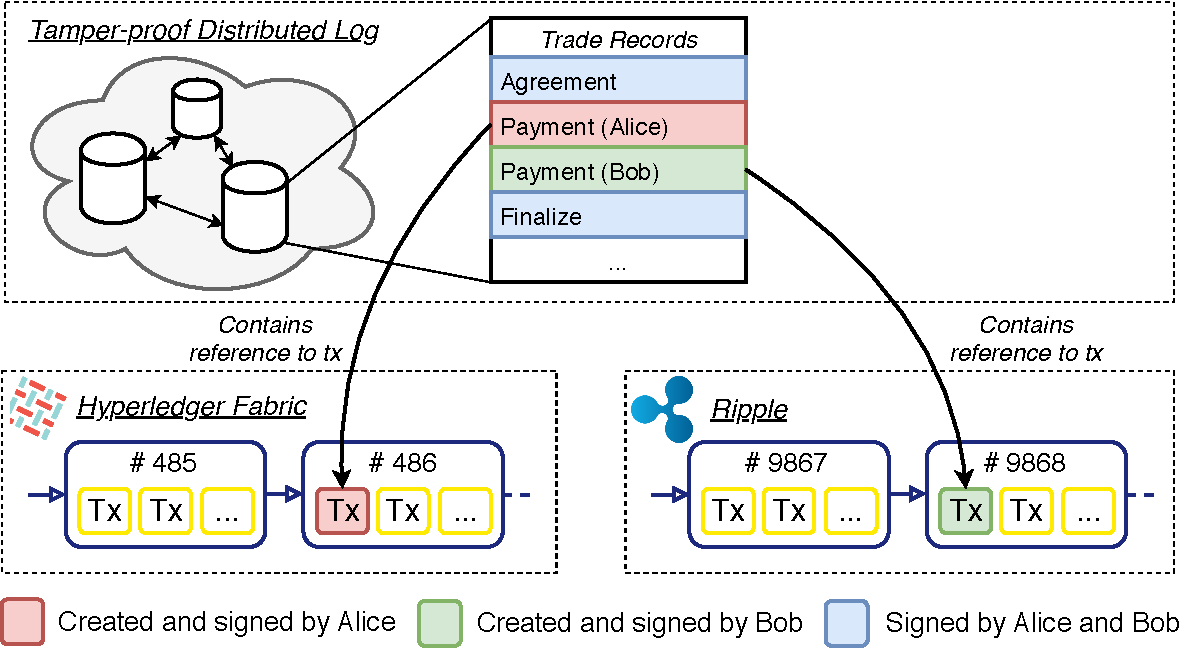
\includegraphics[width=\linewidth]{xchange/assets/xchange}
	\caption{High-level overview of our \ModelName{} trading mechanism. In this example, Alice sells some FabTokens that are managed by Hyperledger Fabric to Bob, who pays Alice in XRP (Ripple) tokens. Full trade specifications are stored in a distributed log.}
	\label{fig:xchange}
\end{figure}

We address fraud concerns by storing trade records in a tamper-proof distributed log.
This distributed log then enables \ModelName{} traders to detect if a party might have committed fraud during an ongoing trade, further discussed in Section~\ref{sec:limit_risk}.
If so, a trader refrains from starting a trade with the suspected party.
We store records of every trade, which makes it difficult for a trader to hide the existence of a specific trade or to unilaterally revert the status of an ongoing trade to a prior state.
Each record in the distributed log is digitally signed by its creator and therefore irrefutably created by a specific peer.
We envision that the distributed log can also be audited by external authorities to resolve potential disputes that would arise during the trade procedure.
However, we consider the details of such audits beyond the scope of this work.
The technical requirements of the distributed log are later discussed in Section~\ref{sec:system_threat_model}.

Before we show how trade specifications are recorded, we first elaborate on two implications of using a shared log.
The first implication is that our solution requires participants to agree on the same distributed log when trading assets using \ModelName{}.
However, in contrast to Internet-of-Blockchains solutions such as Cosmos and Polkadot, \ModelName{} does not require businesses to migrate their deployed ledger applications to a different environment.
Instead, businesses can voluntarily leverage our mechanism and join the \ModelName{} peer-to-peer network without any changes to existing applications.
This approach lowers the adoption barrier of \ModelName{} by interested parties.
The second implication pertains to privacy concerns, arising from the full accounting of trade specifications.
We acknowledge that it might be undesirable to publicly record trade information in specific situations since the records can reveal sensitive business practices.
However, since privacy preservation will likely require additional mechanisms and cryptographic techniques, we consider privacy concerns beyond the scope of our work.

We have considered an alternative design where trade records are stored by the ledgers that are involved in the trade.
Even though this design would avoid the need for a shared log, it would result in the fragmentation of trade records across potentially many different ledgers, making it infeasible to accurately determine in which trades a specific trader is currently involved.
Furthermore, a user can be unable to accurately build profile information of another trader since this user might not have the appropriate credentials to inspect the records and transactions on a specific ledger.
This design would also require logic to store \ModelName{} trade records within all supported blockchain environments, requiring significant implementation efforts.

We show a part of the distributed log in Figure~\ref{fig:xchange} and highlight four records that together describe a completed trade between two traders, Alice and Bob.
This trade exchanges tokens that are managed by a Hyperledger Fabric and a Ripple ledger.
The lower part of Figure~\ref{fig:xchange} shows parts of the Hyperledger Fabric and Ripple ledger.
A completed trade that has been stored in the distributed log consists of the following three record types:

\begin{enumerate}
	\item An \texttt{Agreement} record contains the specifications of an upcoming trade, e.g., the agreed amount of assets that will be exchanged between the traders.
	It also includes information on which party conducts the first payment during the upcoming trade.
	The \texttt{Agreement} record bears the digital signature of both traders and can be appended to the distributed log by any of the traders.
	We further describe this record type, and the other two record types below, in our protocol description (see Section~\ref{sec:protocol}).
	\item A \texttt{Payment} record contains the details of a specific payment that has been conducted during a trade.
	This record includes the identifier of the newly issued transaction that transfers assets in the involved blockchain network.
	For instance, the \texttt{Payment} record created by Alice in Figure~\ref{fig:xchange} contains a reference to the transaction that she submitted in the Hyperledger Fabric network.
	Likewise, the \texttt{Payment} record created by Bob points to his transaction in the Ripple network.
	By including the identifier of the transaction in this record, the trading counterparty, and other traders, can verify if the payer transferred the assets.
	Others can verify the validity and inclusion of the transaction reference by the \texttt{Payment} record by inspecting the appropriate blockchain.
	\item A \texttt{Finalize} record completes a trade.
	A \texttt{Finalize} record is appended to the distributed log by the party that received the last payment during the completed trade.
\end{enumerate}

In addition to these three record types, \ModelName{} also includes the \texttt{Order}, \texttt{CancelOrder}, and \texttt{CancelTrade} records.
The \texttt{Order} and \texttt{CancelOrder} records are used when creating a new order and when canceling an unfulfilled order, respectively.
These two record types are further discussed in Section~\ref{sec:protocol}.
The \texttt{CancelTrade} record can be appended to the distributed log to unilaterally abort the trade if one of the parties becomes inactive during a trade.
This feature is later discussed in Section~\ref{sec:trade-cancellation}.

\subsection{Risk Mitigation}
\label{sec:limit_risk}

%Our solution so far does not address counterparty fraud when exchanging assets.
Even though the distributed log provides traders with an overview of ongoing and finished trades, \ModelName{} does not yet address the situation where a trader conducts \emph{counterparty fraud} during a trade.
As a result, the economic gains of adversaries may be unbounded since a malicious trader can commit fraud in many trades.
Consider a simple trade between Alice and Bob, where Alice sells 2 FabTokens for 40 XRP, and Bob sells 40 XRP for 2 FabTokens.
Both Alice and Bob are expected to individually send their respective assets to each other. 
Since we do not assume atomic exchange, one of the parties, say Alice, has to initiate the first transfer.
As soon as Alice sends 2 FabTokens, she is exposed to \emph{counterparty risk}, as Bob \emph{may not} send back the respective 40 XRP.

In this section we present risk mitigation strategies of \ModelName{} that limit the gains of traders committing counterparty.
These strategies mainly aim at minimizing the assets at stake by dividing each trade into smaller chunks (Section \ref{sec:incremental_settlement}) and by bounding the total amount of obligation a party can enter into (Section \ref{sec:bounded_obligations}).
Throughout the paper, we name the party that is exposed to counterparty risk as \emph{risktaker}, while the other party is called \emph{risky}. 
Determination of the trade roles (who becomes the risky party and who becomes the risktaker) in a prospective trade is explained in Section~\ref{sec:protocol}.


\subsubsection{Incremental Settlement}
\label{sec:incremental_settlement}
The first risk mitigation strategy we introduce is \emph{incremental settlement}, where a trade is incrementally completed in $ k $ near-equal, smaller payments.
Assume that in our fictitious trade between Alice ($ A $) and Bob ($ B $), parties agree to use an incremental settlement with $ k = 2$.
The total trade, therefore, would consist of four consecutive payments as illustrated in Figure~\ref{fig:incremental_trade}. 
Alice is the \emph{risktaker} in this trade and she does the first payment.
Notice that after each payment by Bob, the parties are on par with each other.\footnote{We assume here that a trade exchanges an equal amount of value between both traders. In practice, there are usually small profit margins where one party would gain slightly more in value when the trade is complete.} 
Termination of the trade at this state would not cause an economic loss for any of the parties.
On the other hand, after each payment by Alice, the trade is in a state where Bob has an economic gain of 1 FabToken and Alice experiences an economic loss.
With incremental settlement and $ k = 2 $, Alice is risking only a loss of $ 1 $ FabToken, instead of $ 2 $ FabTokens.
We call the amount of risked assets as the \MarginalStake{}.

Similar to making multiple, smaller payments in the Interledger protocol, traders in \ModelName{} can gradually complete a trade in smaller steps and thus keep the risks manageable.
On the one hand, in a trade where each party transfers value $ v $ to the counterparty, the economic gains of an adversary is reduced to $ \frac{v}{k} $.
On the other hand, incremental settlement prolongs the trade since more payments are made, and as such more transactions must be included on the blockchains that are managing the assets being traded.
In general, a trade completed using incremental settlement requires $ 2k $ \texttt{Payment} records in the distributed log.
In \ModelName{} the value of $ k $ is determined by the risktaker party of the trade and recorded in the \texttt{Agreement} record associated with the trade.

As we experimentally show in Section~\ref{sec:xchange_fraud_experiment}, incremental settlement reduces the value at stake during ongoing trades.
This strategy is not applicable when a trade cannot be completed incrementally, e.g., when exchanging property titles or securities.
Such assets are usually represented by non-fungible tokens on the ledger and gain their value from uniqueness.
Even though these assets cannot be exchanged using incremental settlement, traders can still benefit from the second risk mitigation strategy that bounds the economic gains of adversaries.

We briefly comment on the economic implications of incremental settlement.
Since this approach prolongs the trade duration, it might happen that the price of assets being traded goes in the favour of one of the trading parties.
This is particularly true for high-volatile assets being offered on open, public blockchains.
Price volatility enables the situation where a party can deliberately prolong a trade to profit from price fluctuations.
Ideally, this is something that should be taken into consideration when counterparties create their offer.
We acknowledge that dealing with this economic effect is currently an open issue of our trading system.
At the same time, we believe that this issue is less prominent in permissioned blockchains since the price of such assets are usually not defined by trading volume but rather are priced based on real-world assets (e.g., stablecoins).

\begin{figure}[t]
	\centering
	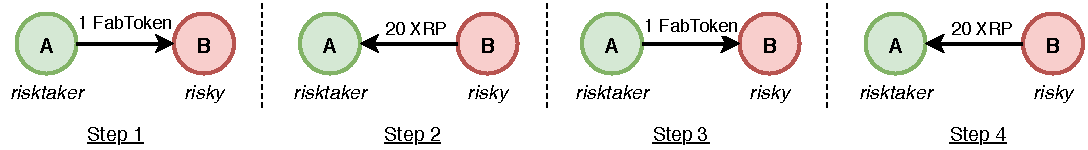
\includegraphics[width=\linewidth]{xchange/assets/trade}
	\caption{An asset exchange with $ k = 2 $ between Alice ($ A $) and Bob ($ B $), trading a total of 2 FabTokens and 40 XRP. During this trade, Alice is the risktaker since she is exposed to counterparty risk. Bob is the risky party since he is able to commit counterparty fraud after step 1 and 3.}
	\label{fig:incremental_trade}
\end{figure}

\subsubsection{Bounded Obligations}
\label{sec:bounded_obligations}
Even though incremental settlement reduces the number of assets the risktaker puts at stake, it does not prevent an adversary from taking part in multiple concurrent trades as a risky party and commit counterparty fraud. 
In the simple trade example above, consider the case where Bob initiated another trade as a risky party with Charlie before finalizing his trade with Alice.
Assume further that both trades are in a state where both Alice and Charlie have made their payments and are waiting for Bob's response. 
There is no restriction for Bob to enter into another trade before fulfilling its trade obligations to Alice and Charlie.

By devising rules that describe when a trader will start a trade with another party, we can bound the economic gains of adversarial parties under the assumption that non-adversarial traders follow the protocol.
We notice that the \emph{risky} party of a trade has no reason to refrain from engaging in an upcoming trade since it has nothing to lose.
A trader becoming a risktaker in a prospective trade, however, must assess the risky party by inspecting the distributed log to determine if it is \enquote{safe} to engage in a trade with it.

One way to mitigate the risk of counterparty fraud would be to forbid a trader from being risky in simultaneous trades.
However, this approach may lead to a situation where a risktaker can arbitrarily delay the trade duration, preventing the risky party to engage in trades with others.
Instead, we choose to bound the \emph{obligations} a trader enters into, by limiting the total amount of \MarginalStake{} within trades where a particular trader is involved in as a risky party.
In other words, \ModelName{} employs trade restrictions which ensure that a malicious trader can only commit counterparty fraud up to a specific value.

In \ModelName{}, every trader $ a $ assigns a \emph{trust threshold} $ u_a(b) $ to every prospective trader $ b $, and refuses to enter into the trade with $ b $ if the total amount of \MarginalStake{} in all \emph{open} trades in which $ b $ is the risky party is larger than $ u_a(b) $. 
Open trades are the ones which do not have a respective \texttt{Finalize} record for its \texttt{Agreement} record in the distributed log.
Formally, given a distributed log $ \mathcal{L} $, let $ P_{\mathcal{L}} $ be the set of all open trades and $ P_{\mathcal{L}}(b) $ be the set of open trades in which trader $ b $ is the risky party. Let $ V(t) $ be the \MarginalStake{} of a trade $ t $.
This value represents how much value a risky party can seize during a trade.
The total value of obligations of a trader $ b $ is referred to as $ B(b) $ and is as follows:

\begin{equation}\label{key}
	B(b) = \sum_{t \in P_{\mathcal{L}}(b)} V(t)
\end{equation}

A trader $ a $ accepts to be a risktaker in a prospective trade $ t' $ with trader $ b $ if the following holds:

\begin{equation}\label{key}
	u_a(b) \geq B(b) + V(t')
\end{equation}

\begin{figure*}[t]
	\centering
	\begin{subfigure}[t]{.4\textwidth}
		\centering
		\captionsetup{width=.9\linewidth}
		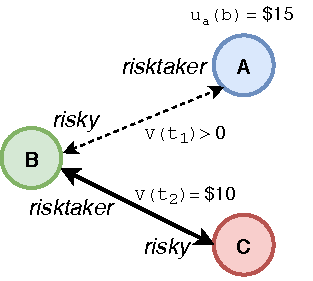
\includegraphics[width=.7\linewidth]{xchange/assets/trade_restriction_1}
		\caption{Trader $ a $ will agree with $ t_1 $ since $ b $ is not risky in any ongoing trade.}
		\label{fig:trade_restriction_1}
	\end{subfigure}%
	\begin{subfigure}[t]{.4\textwidth}
		\centering
		\captionsetup{width=.9\linewidth}
		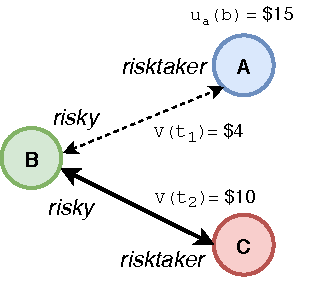
\includegraphics[width=.7\linewidth]{xchange/assets/trade_restriction_2}
		\caption{Total (ongoing + prospective) obligations of $ b $ is smaller than the trust threshold $ u_a(b) $. Trader $ a $ will agree with $ t_1 $.}
		\label{fig:trade_restriction_2}
	\end{subfigure}\vspace{0.5cm}
	\begin{subfigure}[t]{.4\textwidth}
		\centering
		\captionsetup{width=.9\linewidth}
		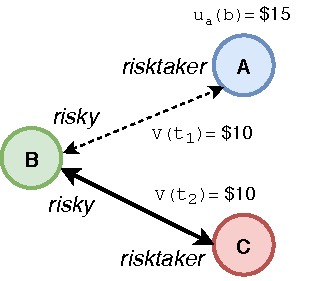
\includegraphics[width=.7\linewidth]{xchange/assets/trade_restriction_3}
		\caption{Trader $ a $ will not agree on $ t_1 $ with since total obligations of $ b $ exceed the threshold. $ a $ and $ b $ may negotiate increasing $ k $.}
		\label{fig:trade_restriction_3}
	\end{subfigure}%
	\caption{Three scenarios in which a trader $ a $ has to decide on starting a prospective trade $ t_1 $ in which $ b $ will become risky. $ a $ agrees with the trade in (a) and (b), and refuses to trade in (c). A solid line represents an ongoing trade whereas a dashed line represents a prospective trade.}
	\label{fig:trade_rules}
\end{figure*}

We illustrate the idea of bounded obligations in Figure~\ref{fig:trade_rules} which shows three scenarios involving traders $ a $, $ b $ and $ c $.  
In all the scenarios, a trader $ a $ has to decide if it wants to start a prospective trade $ t_1 $ with trader $ b $.
We assume that the value of assets involved in trades can be expressed into another asset type, say in United States Dollars (\$).
This conversion could be based on the market price of the involved assets.\footnote{It can also be that traders have differing opinions on the market price of a particular asset, e.g., based on their buy and sell orders.}
The value of \MarginalStake{} in prospective trade $ t_1 $ is \$10, and both parties have agreed that $ a $ becomes the \emph{risktaker} and $ b $ becomes the \emph{risky} if the trade starts.
Trader $ a $ determines a trust threshold $ u_a(b) = \$15 $ for trader $ b $.

Assume $ b $ is already involved in another trade $ t_2 $ with the trader $ c $ and that $ t_2 $ is not finalized.

In Figure~\ref{fig:trade_restriction_1}, trader $ b $ has the role \emph{risktaker} in $ t_2 $.
Since $ b $ is not the risky party in $ t_2 $, it does not have any obligations, i.e., $ B(b) = 0 $.
Therefore, as long as $ u_a(b) > 0 $, trader $ a $ can decide to start a trade with $ b $.
In Figure~\ref{fig:trade_restriction_2} and \ref{fig:trade_restriction_3}, $ b $ is the risky party of $ t_2 $ where $ V(t_2) $ is equal to $ \$4 $ and $ \$10 $, respectively.
In Figure \ref{fig:trade_restriction_2}, trader $ b $'s obligations stemming from ongoing trades amount to \$4, i.e., $ B(b) = 4 $. Since $ b $'s prospective obligations $ V(t_1) + B(b) $ is smaller than the trust threshold, $ a $ agrees to trade with $ b $. 
In Figure~\ref{fig:trade_restriction_3}, the prospective obligations of $ b $ amount to $ \$20 $ and thus exceed the threshold $ u_a(b) $, which would result in the refusal of $ t_1 $ by trader $ a $.
However, even in this scenario, traders may agree to reduce \MarginalStake{} by increasing the $ k $.
Using $ k = 2 $, for example, lowers $ V(t_1) $ to \$5.

%We now introduce three conditions under which a party engages in a trade with another party, based on the records in the distributed log.
%These conditions prevent a party from being risky in multiple high-valued trades at the same time, thus bounding the economic gains of adversaries.
%When following the \ModelName{} protocol, a party $ c $ will only engage in a trade $ T $ with some party $ a $ if at least one of the following three conditions is true:
%\begin{enumerate}
%	\item Trader $ a $ is currently not involved in a trade, \emph{or}
%	\item Trader $ a $ is involved in a trade $ T_{a,b} $ with $ b $ \emph{and} it is currently the responsibility of $ b $ to conduct the next payment in $ T_{a,b} $, \emph{or}
%	\item $ a $ is involved in a trade $ T_1 $ with $ B $ \emph{and} $ A $ is risky in $ T_1 $ \emph{and} $ A $ is willing to become the risktaker in $ T_2 $.
%\end{enumerate}

%We visualize these conditions in Figure~\ref{fig:trade_rules}. 
%In a nutshell, these conditions prevent the risky party to commit counterparty fraud on more than one parties.
%In addition to the above conditions, we note that party $ c $ can always start a trade with another risky party \emph{at its own risk}.
%Condition (1) makes it is safe to engage in asset exchange with a trader that is currently not involved in another trade, see Figure~\ref{fig:trade_1}.
%This condition can be verified by inspection of the distributed log: a party is currently involved in some trade $ T $ when the log contains an \texttt{Agreement} record for $ T $ but no \texttt{Finalize} record for $ T $ (yet).
%Now if all \ModelName{} participants adhere to Condition (1), a malicious trader $ M $ cannot commit counterparty fraud more than once.
%$ M $ would have to successfully complete its ongoing trade to commit fraud with another party, therefore resolving the earlier committed fraud.
%In particular, as long as one of the parties has a responsibility to conduct a payment to the counterparty during a trade, the party waiting for a payment will refuse to sign a \texttt{Finalize} record for that trade.

%If traders in \ModelName{} would only check for Condition (1) when initiating a new trade, both parties of an ongoing trade would be locked out from trading with others until the trade is finalized.
%Conditions (2) and (3) address this situation and enables the risktaker to involve in other trades.
%Conditions (2) and (3) address the case where one of the trading parties becomes inactive.
%For example, during the trade visualized in Figure~\ref{fig:incremental_trade}, Alice can decide not to send the FabToken to Bob before step 1 if she would have second thoughts about the agreed trade.
%Likewise, Bob can decide not to pay Alice the 20 XRP before step 2.
%Under condition (1), both parties are now locked out from trading with others, since other traders detect the incompletion of $ T $.
%This is an unfair situation since the misbehaviour of one party during a trade also negatively affects the other party.
%Even though both parties can become inactive during a trade, there are differences when the risktaker or the risky party becomes inactive.
%If the risky party would become inactive, this situation is considered as counterparty \emph{fraud}, since the inactive party now ends up with a positive economic gain.
%When Bob would become inactive after step 1 or step 3 during the trade visualized in Figure~\ref{fig:incremental_trade}, he would end up with 1 FabToken, without having conducted a corresponding payment back to Alice.
%If the risktaker would become inactive at a specific point during a trade, an equal amount of value has been exchanged between the involved parties.
%When Alice becomes inactive before step 1 or step 3, the trade can be considered as partially complete, and no party would be at a loss.
%Condition (2) defines the circumstances under which a trader $ C $ engages in a new trade $ T_2 $ with another trader that is already a risktaker in an ongoing trade, see Figure~\ref{fig:trade_2}.
%Engaging in a trade with a risktaker does not allow that risktaker to commit fraud in its ongoing trade.
%If party $ A $ would be an adversary, it cannot commit fraud in its ongoing trade $ T_1 $, and therefore, $ A $ cannot commit counterparty fraud in both $ T_1 $ and $ T_2 $, even if $ A $ acts as the risky party in $ T_2 $.
%We remark that the last part of Condition (2) is not strictly required to prevent a malicious party from committing counterparty fraud in multiple trades.
%We have added this logic to discourage $ A $ from becoming inactive in $ T_1 $.
%If $ A $ would become inactive during $ T_1 $ and ends up with the responsibility to conduct the next payment, it has to progress $ T_1 $ before $ T_2 $ takes place.
%This condition can be verified by inspecting the latest \texttt{Payment} record associated with $ T_1 $ in the distributed log.

%Condition (3) defines the circumstances under which a trader $ C $ engages in a new trade with $ A $, while $ A $ is a risky party in an ongoing trade.
%This condition is visualized in Figure~\ref{fig:trade_3}.
%Specifically, $ C $ should only trade with $ A $ if in the upcoming trade $ T_2 $, $ C $ becomes the risky party.
%This prevents $ A $ from becoming risky in both $ T_1 $ and $ T_2 $.
%We remark that all three presented conditions are verified by both parties that intend to trade.
%If $ C $ would already be a risky party in a trade, $ A $ will detects this and as such refuse to trade with $ C $.
%As a consequence of condition (3), two parties that are both risky in different trades never agree to trade with each other.

\subsubsection{Further Comments on Risk Mitigation}
\textbf{Flexible Conformance.} We note that a trader can always ignore the risk mitigation strategies described in this section and engage in other trades \emph{at its own risk}.
Doing so, however, does not provide restrictions on the economic gains of adversarial parties but it enables participants to engage in trade with traders with which there is an existing trust relation (e.g., the traders know each other in real life).
Trades that parties started at their own risk do not impact the obligations of the risky party in such trades.
Such trades contain a special flag in the associated \texttt{Agreement} record.

\textbf{Subjectivity and Trust.} We note that the threshold function $ u_a $ is a subjective matter for a trader $ a $ and is highly dependent on the notions of trust and reputation, which are outside the scope of our work.
Without loss of generality and for simplicity, we assume in the rest of the paper that $ u_a(b) $ is equal to a constant $ U $ for all trader pairs $ a $ and $ b $.

\textbf{Determination of $ k $.} 
Parameter $ k $ signifies the number of payments each party does in a trade.
This value is proposed by the risktaking party during trade negotiations and is included in the \texttt{Agreement} record in the distributed log.
We note that both sides of a trade are concerned with the value of $ k $.
For the risktaker, $ k $ determines the \MarginalStake{}, i.e., the value that the risktaker may lose in case of counterparty fraud by the other party.
For the risky party, $ k $ affects the maximum rate of trade a party can be involved in as a risky party.
While lowering the value of $ k $ brings together low-risk advantage for the risktaker and trust advantage for the risky party, it, in return, increases the duration of a trade, i.e., the number of transactions needed to settle the trade.

%We call the value $ u_a(b) - B(b) $ as the \emph{trading residue} of trader $ b $ with respect to $ a $, and denote this by $ D_{a,b} $.
%In essence, the trading residue denotes how much tolerated opportunity for fraud a trader $ b $ has from the perspective of $ a $.
%Before $ a $ agrees to trade with $ b $, $ a $ determines the trading residue of $ b $ using the records in the distributed log, and then determines if starting the prospective trade would exceed the trading residue.

%Trader $ a $ will also take into consideration the incremental settlement strategy when the trading residue of $ b $ is low, which will decrease the value of $ V(T_{a,b}) $.

\subsection{Cancellation of a Trade}
\label{sec:trade-cancellation}
We note that a trade may never complete if a risktaker goes offline.
The total amount of \MarginalStake{} in all such \emph{stalled} trades in which a party $ b $ is a risky party may reach a point where no-one wants to trade with $ b $, even if $ b $ is not at fault.
Therefore, the ability of a trader $ b $ to trade with others may be forever restricted.
To address this situation, we allow a risky party to explicitly cancel an ongoing trade by including a \texttt{CancelTrade} record in the distributed log.
This record can only be included by the risky party, and is only acknowledged by other traders if (1) the risktaker is currently responsible for transferring assets to the risky party during the trade, and (2) at least some time $ \Delta_t $ has elapsed since the last activity in trade $ t $.
The value of $ \Delta_t $ should be well above the confirmation times of transactions submitted to the involved blockchains, to avoid the situation where one might consider a trade as stale while a transaction is still being finalized in the involved blockchain.
When a trade is cancelled, no other assets should be exchanged.
After the risky partner cancelled participation in a trade, it loses its risky status and can then participate in other trades.

We note that a risky party $ a $ can try to trick another party $ b $ into acknowledging a \texttt{CancelTrade} record by publishing a \texttt{Payment} record with a non-existent transaction identifier.
Therefore, $ b $ needs to inspect the involved ledger to determine the validity of a \texttt{CancelTrade} record created by $ a $.
However, $ b $ might not have the appropriate credentials to read transactions on this ledger.
Even though the \texttt{CancelTrade} transaction might be valid, we assume that $ b $ will not acknowledge the \texttt{CancelTrade} record when it cannot accurately determine its validity.
We argue this is reasonable since this particular situation is likely to be infrequent.
We also believe that this design decision does not significantly limit the efficiency of our mechanism.

%It might be that $ C $ does not have the appropriate credentials to read transactions in $ \mathcal{B}_a $ or $ \mathcal{B}_b $, and therefore is unable to determine if a \texttt{Payment} or \texttt{CancelTrade} record by party $ A $ is legitimate.
%If $ C $ is unable to determine the legitimacy of the trade record, $ C $ refuses to trade with $ A $, since the claims of $ A $ cannot be accurately verified.
%This issue could be resolved by having a special peer, or \emph{gateway}, for each connected blockchain that can be queried by traders when one wants to verify the existence and validity of a transaction on a particular blockchain.
%We consider the question on how to build such a gateway beyond the scope of this work.

%We summarize and visualize the three presented conditions in Figure~\ref{fig:trade_rules}.


%\subsection{Fraud Tolerances}
%\label{sec:determining_fraud_tolerance}
%Each trader maintains a value $ U $ that indicates the maximum value with which a trader trust a trading counterparty.\todo{fraud tolerance is not the right word}
%As we will prove in Section~\ref{sec:analysis}, if every trader uses a fixed value for $ U $, the economic gains of adversaries is bounded by $ U $.
%However, traders can use different values of $ U $ for different traders.
%For example, if a counterparty $ b $ has successfully completed high-valued trades in the past, a trader $ a $ can increase the value of $ U_{a,b} $.
%We suggest that the value of $ U $ is guided by a reputation algorithm, e.g., by taking the historical trades of trading counterparties into consideration.

%\subsection{Accurate Trade Inspections}
%Our solution described so far requires other traders to verify whether a specific trader is currently involved in a trade and, if so, if it is their responsibility to conduct the next payment during this trade.\todo{rewrite!}
%However, a trader can create a \texttt{Payment} record that includes the identifier of a non-existent or invalid transaction in the involved blockchain.
%Therefore, traders cannot accurately decide the current state of a trade merely based on the records in the distributed log since a trader can make false claims.
%In some situations, traders must perform an additional verification step by inspecting the validity of a transaction on connected blockchains.
%Suppose an ongoing trade $ T $ between $ A $ and $ B $, where $ A $ sells some assets $ a $ and $ B $ sells some assets $ b $.
%These assets are managed by blockchains $ \mathcal{B}_a $ and $ \mathcal{B}_b $, respectively.
%Now, to verify whether a trader $ C $ can open a trade with $ A $, a trader has to inspect the validity of a particular transaction in $ \mathcal{B}_a $ or $ \mathcal{B}_b $ in the following two situations:

%\begin{enumerate}
%	\item The latest record associated with $ T $ in the distributed log is a \texttt{Payment} record.
%	To verify that the creator of this record conducted the payment, $ C $ has to verify the existence and validity of the transaction to which the \texttt{Payment} record points.
%	\item The latest record associated with $ T $ in the distributed log is a \texttt{CancelTrade} record.
%	$ C $ has to verify that the creation of this record adheres to the trade cancellation rules that we discussed in Section~\ref{sec:limit_risk}.
%	To determine this, $ C $ potentially has to check the validity of the latest \texttt{Payment} record associated with $ T $.
%\end{enumerate}

% Key insight: only one party can effectively commit fraud, depending on who "goes first"
% This party is called risky. For each trade, there is a risky and a non-risky party.
% A counterparty can explicitly cancel a trade if it falls victim to griefing.
% A risky party can remove its risky status by:
%		1) completing the trade
%		2) completing its obligations to the counterparty, putting the trade in a "neutral" state, and posting a "cancel" transaction.

% Someone will always trade with someone else that is not involved in a trade.
% When will someone trade with a non-risky party A?
%		When there is recent progress by A (an outgoing payment)
% When will someone trade with a risky party B?
%		If it is the responsibility of A to act in a trade (requires deep trade inspection)

%\begin{enumerate}
%\item \textbf{Limit the number of ongoing trades}. In \ModelName{}, a trader will only engage in a trade with some counterparty $ c $ if $ c $ is either not currently involved in a trade with another party, or the ongoing trade involving $ c $ is \emph{stale}, and trade staleness is not due to $ c $.
%A stale trade in the context of \ModelName{} is a trade that has not progressed for a pre-defined amount of time, and where it is likely that one of the parties is either offline or has compromised assets from the trading counterparty.
%Before one can engage in another trade, they must finish its ongoing trade first.
%This restriction acts as a punishment for adversarial parties since it prevents further economic activity until their current trade has been completed.
%Since we assume well-established identities (see Section~\ref{sec:system_threat_model}), an adversarial trader cannot easily re-enter the network under a different identity.
%If $ c $ nonetheless is able to convince multiple traders to engage in a trade, integrity constraints enforced by the blockchain will ensure that $ c $ can only start a single trade.
%We remark that a trader can still start a trade \textit{at its own risk} with a party currently involved in another trade.
%This enables high-reputed traders to engage in multiple trades at once.
%\end{enumerate}

%The implementation of the \ModelName{} trading mechanism compromises of a five-phase trading protocol and a system architecture.
%The formal specifications of the trading protocol are given in the next section whereas the system architecture of \ModelName{} is elaborated in Section~\ref{sec:architecture}.

\section{System Assumptions and Threat Model}
\label{sec:system_threat_model}
We first discuss the \ModelName{} system model.
This includes our assumptions on the blockchains that are managing the assets being exchanged, the requirements of the distributed log used by \ModelName{}, and the specifications of the underlying \ModelName{} network.
We then present the threat model of \ModelName{}, and state the goals and capabilities of adversarial parties.

\subsection{Blockchain, Distributed Log, and Network Specifications}
\label{sec:blockchain_network_specs}
The \ModelName{} mechanism coordinates asset exchange between permissioned blockchains.
W.l.o.g., we denote the blockchains that are managing the assets being exchanged by $ \mathcal{B}_a $ and $ \mathcal{B}_b $ respectively.
\ModelName{} only requires that $ \mathcal{B}_a $ and $ \mathcal{B}_b $ can represent assets and transfer assets to another owner.
The consensus mechanisms deployed by $ \mathcal{B}_a $ and $ \mathcal{B}_b $ might be fundamentally different.
We assume that for each involved blockchain, the fraction of adversarial parties is bound by the threshold necessary to ensure safety and liveness properties.
In PBFT-based consensus algorithms, this threshold is usually $ \frac{1}{3} $ of all nodes involved in the consensus algorithm~\cite{castro1999practical}.

\ModelName{} stores trade records in a distributed log, denoted by $ \mathcal{L} $.
We require that the entries stored by $ \mathcal{L} $ are immutable and append-only.
If entries in $ \mathcal{L} $ would be mutable or can be removed, a trader could trick a counterparty into starting a trade, commit counterparty fraud, and remove all traces of the trade.
Similar to how participation in $ \mathcal{B}_a $ and $ \mathcal{B}_b $ is explicitly approved, participation in $ \mathcal{L} $ should be managed by an authority.
We envision that a trader joining \ModelName{} re-uses the well-defined identity under which it participates in one of the permissioned blockchains.
We remark that $ \mathcal{L} $ can, for example, be realized through a blockchain with support for smart contracts.

Users in \ModelName{} participate in a peer-to-peer network, which is used to send point-to-point messages to other users.
This network is particularly used during trade negotiation, as we further specify in Section~\ref{sec:protocol}.
We assume that peers in the \ModelName{} network know the network addresses of other peers.

\subsection{Peer Model}
We now elaborate on the assumptions of peers participating in \ModelName{}.

Each peer in the \ModelName{} network owns a cryptographic key pair consisting of a public and a private key. 
The public key of a specific peer is known to others and uniquely identifies it in the network. 
Their private key is used to digitally sign data such as records appended to $ \mathcal{L} $, or outbound messages in the peer-to-peer network.

As we discussed in Section~\ref{sec:blockchain_network_specs}, the digital identity of each peer in the \ModelName{} network uniquely identifies a real-world user.
Identity validation should be performed by a Registration Authority (RA), which is external to our system.
The RA could be the same authority that approved participation in $ \mathcal{B}_a $ or $ \mathcal{B}_b $.
We assume that the RA does not collude with traders in \ModelName{}.
In \ModelName{}, well-established digital identities are necessary to prevent misbehaviours such as a Sybil Attack and a distributed denial-of-service attack~\cite{douceur2002sybil,Specht2004DistributedDO}.
We also use verified identities for accountability purposes, where misbehaviour in a trade can be traced back to a real-world persona.

Whereas existing work primarily focuses on \emph{how} assets are exchanged, the \ModelName{} mechanism also includes primitives for traders to specify trade interest through orders, and to find trading partners that can fulfil these orders.
We distinguish between \emph{makers} and \emph{takers}.
A maker is a peer that creates a specific order, whereas a taker is a peer that fulfils an order.
Makers introduce trading opportunities and liquidity to the \ModelName{} network.
A peer in \ModelName{} can act as both maker and taker, for distinct orders.
The maker-taker order model is also adopted by related protocols that enable the exchange of tokens on the Ethereum blockchain, namely 0x and AirSwap~\cite{warren20170x,airswap}.
System designers can also consider to leverage more advanced decentralized matchmaking solutions, e.g., as described in our prior work~\cite{vos2020match}.

\subsection{Threat Model}
Adversarial parties in \ModelName{} aim to \emph{maximize their economic gains} by committing counterparty fraud in ongoing trades.
Adversarial parties could attempt to append invalid records to $ \mathcal{L} $, intentionally ignore incoming messages in the peer-to-peer network, or refuse to respond to messages during trade negotiation.
They also could strategically ignore the risk mitigation strategies described in Section~\ref{sec:limit_risk}.
We assume that adversaries cannot compromise the integrity of the distributed log $ \mathcal{L} $ used by \ModelName{} and cannot undermine the security of the blockchains that are hosting the assets being traded, $ \mathcal{B}_a $ or $ \mathcal{B}_b $.
We also assume that the cryptographic primitives used by all involved blockchains are secure (e.g., digital signatures cannot be forged) and that the computational capabilities of adversaries are bounded.

\section{The \ModelName{} Trading Protocol} \label{sec:protocol}
We now present the \ModelName{} trading protocol for asset exchange between permissioned blockchains and specify all operations conducted by peers that are participating in a trade.
We assume the system and threat model described in the prior section.
The protocol consists of four phases.
In the first phase, makers specify their trade interest by appending new orders to the distributed log $ \mathcal{L} $.
During the second phase, takers negotiate with makers about orders they would like to fulfil and append an \texttt{Agreement} record to the distributed log when they reach an agreement.
During the third phase, the maker and taker execute the trade by exchange assets through payments.
The trade is finalized in the fourth phase with a \texttt{Finalize} record.

\begin{figure}[h]
	\centering
	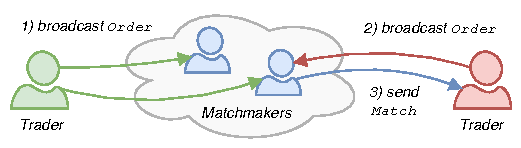
\includegraphics[width=0.7\linewidth]{xchange/assets/xchange_protocol_1}
	\caption{Phase I of the \ModelName{} trading protocol: makers (depicted in green) indicate trade interests by appending an \texttt{Order} record to the distributed log.}
	\label{fig:matching_protocol_1}
\end{figure}

\subsection*{Phase I: Order Creation and Cancellation}
\label{sec:phase_matching}

During the first phase of the \ModelName{} protocol, makers create new orders and append these orders to $ \mathcal{L} $, see Figure~\ref{fig:matching_protocol_1}.
When a trader intends to buy or sell some assets, it constructs a new order which we denote by $ O $.
$ O $ contains details on the quantity and the type of assets that the maker desires to buy and sell.
The order creator provides this information as a two-tuple of asset quantities, also called an \emph{asset pair}.
The first asset quantity in the asset pair indicates the assets that the order creator wants, and the second asset quantity indicates what the order creator offers in return.
An asset quantity is described by the combination of an integer value and a string that indicates the asset type.
For example, if a trader intends to sell 2 FabTokens for 40 XRP tokens, it creates an order with asset pair ($ 2 $ FabToken, $ 40 $ XRP).

$ O $ includes an integer value, $ k $, that specifies the order creator's preference regarding the number of partitions each payment is divided in.
As discussed in Section~\ref{sec:incremental_settlement}, one way how \ModelName{} reduces value at stake is by using incremental settlement.
The inclusion of $ k $ in $ O $ indicates the risk that the maker is willing to take in an upcoming trade that fulfils $ O $ if the order creator would become the risktaker.
Furthermore, $ O $ includes the address of the wallet in which the order creator wishes to receive assets from a prospective trader during an upcoming trade.
By including this information, a taker knows to which address it should transfer its assets.
This information is also used by other traders to verify if the maker has received assets from a taker.

%We observe that a maker may create a \enquote{fake} order that specifies interest to sell assets that the maker does not possess.
%Essentially, this order provides non-existent liquidity to the \ModelName{} network, since a trade fulfilling the fake order will never complete.
%We address the creation of orders that are not backed by real assets by requiring a \emph{proof-of-ownership} in each new order.
%A proof-of-ownership proves that a specific peer holds ownership over assets managed by some blockchain $ \mathcal{B}_a $.
%This proof is represented as a combination of a public key and a digital signature over the order content in serialized form.
%To generate this signature, the order creator should use the cryptographic key pair associated with the account on $ \mathcal{B}_a $ that holds the assets that the order creator intends to sell.
%Takers verify the proof-of-ownership to check that the order creator could complete a prospective trade, and owns the assets it intends to sell.

After adding all required fields to $ O $, the order creator serializes the order and embeds it in an \texttt{Order} record.
The order creator then appends the \texttt{Order} record to $ \mathcal{L} $.
The order identifier can be determined by taking the hash of the record content, which we denote by $ H(O) $.

A maker can cancel any of their non-expired orders that are not being fulfilled by an ongoing trade.
This is achieved by the maker appending a \texttt{CancelOrder} record containing $ H(O) $ to $ \mathcal{L} $.

\begin{figure}[h]
	\centering
	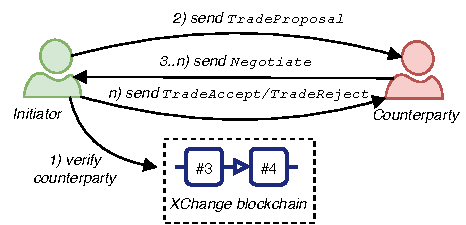
\includegraphics[width=0.7\linewidth]{xchange/assets/xchange_protocol_2}
	\caption{Phase II of the \ModelName{} protocol: a maker and taker negotiate a trade agreement. Upon a successful negotiation outcome, a dual-signed \texttt{Agreement} record will be appended to the distributed log.}
	\label{fig:matching_protocol_2}
\end{figure}

\subsection*{Phase II: Trade Negotiation}
\label{sec:phase_clearing}

During the second phase of the \ModelName{} trading protocol, a maker and taker negotiate a trade, see Figure \ref{fig:matching_protocol_2}.
If the negotiating maker and taker agree to trade, one of the parties appends this agreement to $ \mathcal{L} $.
We now describe this negotiation process.

This phase starts when a taker discovers an order $ O $, included on $ \mathcal{L} $, that it wishes to fulfil.
Assume that this order has been created by a maker $ M $.
Before sending a trade proposal to $ M $, the taker performs two checks that determine if the taker should trade with $ M $.
First, the taker checks if it is willing to trade with $ M $ as a person.
For instance, $ M $ could have attempted to commit counterparty fraud in the past, which could be a reason for the taker to refrain from trading with $ M $.
Second, the taker determines if it is safe to trade with $ M $, according to the \emph{bounded obligations} strategy described in Section~\ref{sec:bounded_obligations}.
The taker checks the trades in which $ M $ is involved by inspecting the latest records on $ \mathcal{L} $ involving $ M $.
If $ M $ is already involved in a trade $ T $, the information on $ \mathcal{L} $ also reveals if $ M $ in $ T $ is a risky party or a risktaker.

When both checks pass, the taker creates and sends a \texttt{Proposal} message to $ M $.
A \texttt{Proposal} message contains a proposal for $ M $ to fulfil order $ O $.
A taker includes four pieces of information in a \texttt{Proposal} message.
First, it includes the identifier of $ O $, so the maker knows which order the taker wants to fulfil (a trader could have created multiple orders).
Second, the taker includes its destination wallet address to which $ M $ should send its assets during the trade.
Third, the taker includes an integer value, $ k $, that indicates how much risk the taker is willing to take if it would become the risktaking party.
Finally, the taker includes a boolean value in the proposal indicating if the taker becomes a risktaker in the upcoming trade.
At a high level, a \texttt{Propose} message represents a new order that indicates the taker's trade preferences.

When $ M $ receives a \texttt{Proposal} message from taker $ T $, it also verifies whether it wants to trade with $ T $.
Specifically, $ M $ performs the same two checks as the taker did.
Furthermore, $ M $ verifies if it agrees with the role classification proposed by the taker.
If validation fails, the maker immediately sends a \texttt{Reject} message back to the taker, containing the identifier of the rejected order and, optionally, why $ M $ has rejected the proposal.
If $ M $ agrees with the proposal and also wishes to trade with $ T $, $ M $ constructs a \texttt{Agreement} record, which includes the identifier of the order being fulfilled and the proposal created by the taker (including the taker's signature).
This \texttt{Agreement} record is signed by $ M $, sent back to $ T $, and appended to $ \mathcal{L} $.
Inclusion of the \texttt{Agreement} record on $ \mathcal{L} $ binds the maker and the taker to the trade agreements.
Since the risktaker is exposed to counterparty risk in the upcoming trade, the preferred value of $ k $ by the risktaker is used during the upcoming asset exchange.
If the maker is the risktaker, the value of $ k $ as specified in the \texttt{Order} record describing $ O $ is leading.
Otherwise, if the taker becomes the risktaker, the value of $ k $ specified by the taker in its proposal is leading.

\begin{figure}[h]
	\centering
	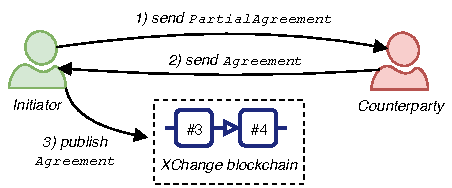
\includegraphics[width=0.8\linewidth]{xchange/assets/xchange_protocol_3}
	\caption{Phase III of the \ModelName{} protocol: a maker and taker trade by exchanging assets. In this trade, the taker is the risktaker (initiating the first payment) and the maker is the risky party.}
	\label{fig:matching_protocol_3}
\end{figure}

\subsection*{Phase III: Trade Settlement}
\label{sec:phase_settlement}
During the third phase of the \ModelName{} trading protocol, assets are exchanged between the maker and taker, and the trade is settled.
Figure~\ref{fig:matching_protocol_3} visualizes a trade between a maker and taker, with $ k = 1 $, where the maker sells FabTokens, a token managed by Hyperledger Fabric, and gets XRP (Ripple) tokens in return from the taker.
This trade, fulfilling order $ O $, consists of two payments, one from the maker to the taker, and one from the taker to the maker.

Asset exchange starts by the risktaker (the taker in this specific example) issuing a transaction to the Ripple network managing the XRP tokens.
This Ripple transaction transfers XRP tokens from the wallet specified in the \texttt{Proposal} message to the wallet address that was specified by the maker in the \texttt{Order} record associated with $ O $.
After the taker has issued this transaction in the Ripple network, it appends a \texttt{Payment} record to $ \mathcal{L} $, which contains the identifier of the order being fulfilled, and the identifier of Ripple transaction.
The \texttt{Payment} record allows the maker (and other traders) to verify that the taker has transferred the correct amount of assets to the maker.

After the maker has verified that it received the agreed amount of XRP tokens, it conducts the next payment by issuing a transaction to the Hyperledger Fabric network.
This transaction transfers FabTokens from the wallet specified in the \texttt{Order} record to the wallet that was specified by the taker in the \texttt{Proposal} message.
The maker then appends a \texttt{Payment} to $ \mathcal{L} $, which includes the identifier of the transaction in the Hyperledger Fabric network.
This payment process repeats until all assets have been exchanged between the maker and the taker.

There is a risk that a trade does not progress when one of the traders becomes inactive.
As pointed out in Section~\ref{sec:limit_risk}, a stale trade is only a minor concern for the risktaker since this party can still engage in other trades after $ \Delta_T $ time has elapsed.
A risky party can explicitly cancel an ongoing trade to dismiss its responsibility as a risky party by appending a \texttt{CancelTrade} record to $ \mathcal{L} $.
This record only contains the identifier of the order currently being fulfilled.
Other traders should verify that the \texttt{CancelTrade} adheres to the rules as outlined in Section~\ref{sec:limit_risk}, to prevent the risky party from illegally cancelling a trade after having committed counterparty fraud.

\begin{figure}[h]
	\centering
	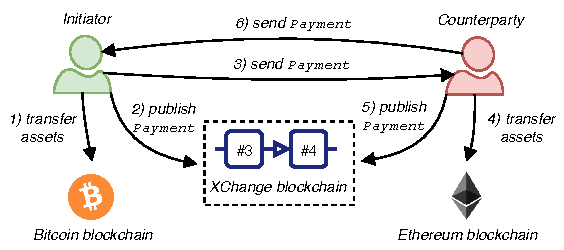
\includegraphics[width=0.7\linewidth]{xchange/assets/xchange_protocol_4}
	\caption{Phase IV of the \ModelName{} protocol: the taker finalizes the trade.}
	\label{fig:matching_protocol_4}
\end{figure}

\subsection*{Phase VI: Trade Finalization}
\label{sec:phase_finalization}
When all assets have been exchanged, the party receiving the final payment during a trade creates a \texttt{Finalize} record and appends it to $ \mathcal{L} $, see Figure~\ref{fig:matching_protocol_4}.
Since the risky party conducts the final payment during a trade, finalization is always performed by the risktaker.
Inclusion of a \texttt{Finalize} record on $ \mathcal{L} $ completes a trade, say $ T_1 $, between the maker and taker, and both parties can now start new trades with others.
%One might argue that an explicit finalization is redundant since a trader can determine if $ T_1 $ is complete by counting the number of issued \texttt{Payment} records during the trade.
%However, the risky party might include a \texttt{Payment} transaction without actually having transferred the assets, which can falsely trick other users into thinking that the trade has been successful.
%A \texttt{Finalize} record indicates that the trade has explicitly been finished by both parties and that both parties acknowledge that the trade is complete.
%Note that if the risktaker waits too long with submitting a \texttt{Finalize} record after a trade has been complete, it is considered as griefing after some time has elapsed.

\section{Security Analysis}
\label{sec:analysis}
We now analyse the security of the \ModelName{} mechanism.
First, we prove that the economic gains of adversarial parties committing counterparty fraud are upper-bounded.
We then discuss the scenario where multiple adversaries collude to gain an advantage as a group.

\subsection{Counterparty Fraud Limitations}
We further analyse the \emph{bounded obligations} strategy presented in Section~\ref{sec:bounded_obligations}.
This strategy define an upper bound on the obligations an adversary can enter into, under the condition that all honest traders act rationally and try to minimize their risk.

\textbf{Limiting the Gains of Adversaries.} 
To show that \ModelName{} limits the amount of fraud, we assume  ---for clarity--- that all honest peers fix a unit trust threshold $ U $, and the number of payments in each trade $ t $ is fixed to $ K $. 
Specifically, where $ P $ is the set of traders and $ T $ is the set of all trades, the following is assumed:
\begin{equation*}
	(u_i = U) \quad\forall i\in P \quad\text{ and }\quad (k_j = K) \quad\forall j \in T.
\end{equation*}

Under these two assumptions, \ModelName{} guarantees that:

\begin{itemize}
	\item[(1)] the total value of assets an adversary can gain as result of counterparty frauds is limited to $ U $,
	\item[(2)] the loss of an honest party in a trade is limited to $ V/K $, where $ V $ is the \MarginalStake{} during the trade.
\end{itemize}

Assume an adversarial trader $ B $ is involved in $ (n-1) $ trades denoted by $ t_1, t_2, \ldots, t_{n-1} $ in which $ B $ is the risky party and is in trade negotiations with an honest trader $ A $ for the prospective trade $ t_n $.
Assume $\sum_{i \in \{1, \ldots, n-1\}} V(t_i) \leq K\cdotp U$ and $\sum_{i \in \{1, \ldots, n\}} V(t_i) > K\cdotp U$.
Under these conditions, trader $ A $ does start a trade with $ B $, given that $ A $ follows \ModelName{} protocol.

We can now show the correctness of the statement (1) and (2) above.
There are two ways a malicious party can commit counterparty fraud.
Firstly, it can choose to become inactive in a trade and not conduct a payment back to the risktaker.
Secondly, $ B $ could append a \texttt{Payment} record to $ \mathcal{L} $ that points to a non-existent or invalid transaction, attempting to trick the risktaker counterparty and other traders.
In both cases, the value of fraud in a trade $ t $ cannot exceed $ V(t)/K $, which verifies statement (2).
Therefore, even when we assume that $ B $ commits counterparty fraud in all the active trades it is involved, the total value of assets $ B $ can gain does not exceed $ U $, which verifies statement (1). 

We can now relax our assumptions on the objectivity of trust threshold $ (U) $ and the number of payments $ (K) $.
Assuming each trade $ t $ has its own number of payments $ k_t $ agreed by the trading parties, the amount of assets the risktaker can lose in $ t $ is limited by $ V(t)/k_t $.
When $ u_A(B) $ is the trader $ A $'s subjective trust threshold assigned to trader $ B $, then trader $ A $ does not start a trade $ t $ with $ B $ if the existing obligations of $ B $ exceed $ u_a(b) - V(t)/k_t $.
Assuming $ k_t $ is not bounded and that $ V(t)/k_t $ may converge to zero, a trader $ B $ can start a trade as a risky party with a trader $ b $, only if its obligations occurred from ongoing trades is limited by $ u_a(b) $.
Accordingly, defining $ \bar{u} = \max\{u_j(b) : j\in V\} $ where $ V $ is the set of all prospective traders with $ b $, the total amount of assets that $ b $ can seize in \ModelName{} cannot exceed $ \bar{u} $.

\textbf{Limit on the Risktaker's Loss.} 
In \ModelName{}, the risktaker's loss in a single trade is bounded with the trust threshold $ u $ associated with the risky party.
Furthermore, as the risktaker is involved in the determination of number of payments ($ k $) during trade negotiations, it can reduce its own risk to any extent.
Nevertheless we note that \ModelName{} does not introduce a theoretical bound on the loss of a risktaker over time, but delegates the risk management to the risktaker by assuming a trust mechanism to determine the trust threshold.
Specifically, \ModelName{} provides the risktaker with two important parameters $ u $ and $ k $ with which the risktaker can minimize its own risk, relying on the trust mechanism.

\textbf{Malevolent Cancellation of a Trade.} 
We now analyse the situation where a risky party $ B $ cancels its ongoing trade $ t_1 $ with $ A $ by appending a \texttt{CancelTrade} record to $ \mathcal{L} $, before the trade is finalized and when it is $ B $'s turn to make payment.
When a third party $ C $ considers entering in trade $ t_2 $ with $ B $, it will discover the \texttt{CancelTrade} record in $ \mathcal{L} $ and check whether the trade cancellation by $ B $ is legitimate (see Section \ref{sec:trade-cancellation}).
Recall that the cancellation of a trade by $ B $ is legitimate if it is currently the responsibility of the risktaker to conduct the next payment.
The trade cancellation of $ t_1 $ is therefore not valid since $ B $ has committed counterparty fraud.
If the trade cancellation were legit, $ B $ would not have been under no obligation in trade $ t_1 $, since it would have transferred assets to $ A $.
Now, when $ C $ verifies the status of $ B $ and detect an illegitimate trade cancellation, $ C $ will not engage in trade $ t_2 $ with $ B $.

\subsection{Collusion Resistance}
In a collusion attack, a group of traders follows a common strategy to subvert the network or gain advantages as a collective.
The \ModelName{} mechanism is highly resistant against collusion attacks since adversarial parties are not able to gain more economic gains when working together, given that $ \mathcal{L} $ provides secure storage of included trade records.
We argue that the resistance against collusion can be addressed to the absence of group-based coordination in \ModelName{}.
Tasks that would involve coordination among a group are usually vulnerable to attacks where a majority of the group colludes to gain advantages over non-colluding users.
In \ModelName{}, trade proceeds through the direct interaction between the involved traders and therefore, cannot be influenced by groups of colluding adversaries.

\section{Distributed Logging of Trade Records}
\label{sec:blockchain_accounting}
The \ModelName{} trading protocol described in Section~\ref{sec:protocol} requires a distributed log to securely and irreversibly store \texttt{Order}, \texttt{CancelOrder}, \texttt{Agreement}, \texttt{Payment}, \texttt{Finalize} and \texttt{CancelTrade} records.
We choose to build \ModelName{} upon TrustChain~\cite{otte2017trustchain} which is a shared data structure with a sharp focus on tamper-resilience and trustworthy record storage.
In this section we motivate our choice for TrustChain and outline how TrustChain is used to store \ModelName{} records.\footnote{The TrustChain architecture described in this chapter is an earlier version of \TrustChain{}, which has been presented in Chapter~\ref{chapter:trustchain}.}

\subsection{TrustChain: A Scalable Ledger for Accounting} \label{sec:trustchain}
Based on the idea of blockchain ledgers that order transactions in a directed acyclic graph (DAG), Otte et al. designed, implemented, and deployed TrustChain.
TrustChain is a ledger that is optimized for lightweight, tamper-proof accounting of data elements~\cite{otte2017trustchain}.
The key idea is that individuals maintain and grow their \emph{individual ledger} with records.
Other users verify these records according to some pre-defined rules.
This makes TrustChain similar to solutions for tamper-proof, distributed logging, such as PeerReview~\cite{haeberlen2007peerreview}.
TrustChain does not aim to prevent integrity attacks on the data structure, e.g., fork creation, but instead guarantees eventual \emph{detection} of these attacks.
This yields superior scalability compared to other ledgers but allows for the situation where some malicious activity targeted at the ledger might go undetected for some time, for example, the hiding of specific transactions.
In TrustChain, this can be addressed by waiting longer before accepting a record as valid.
Individuals in TrustChain are not required to store all records in the network and might choose to store different parts of the global DAG ledger.
TrustChain does not reach a global consensus over all records but relies on participants to detect inconsistencies in individual ledgers.

\begin{figure*}[t]
	\centering
	\begin{subfigure}[t]{.45\textwidth}
		\centering
		\captionsetup{width=.9\linewidth}
		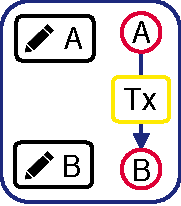
\includegraphics[width=.35\linewidth]{xchange/assets/trustchain_tutorial_1}
		\caption{A block with a record (\emph{R}) between two users ($ A $ and $ B $). Each block contains a single record, two digital signatures and two digital identities.}
		\label{fig:trustchain_tutorial_1}
	\end{subfigure}%
	\begin{subfigure}[t]{.45\textwidth}
		\centering
		\captionsetup{width=.9\linewidth}
		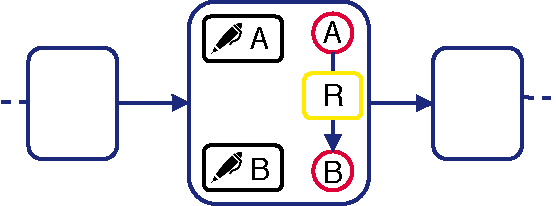
\includegraphics[width=\linewidth]{xchange/assets/trustchain_tutorial_2}
		\caption{An individual ledger. Each block in the chain contains a hash that describes the prior block.}
		\label{fig:trustchain_tutorial_2}
	\end{subfigure}
	\par\bigskip
	\begin{subfigure}[t]{.45\textwidth}
		\centering
		\captionsetup{width=.9\linewidth}
		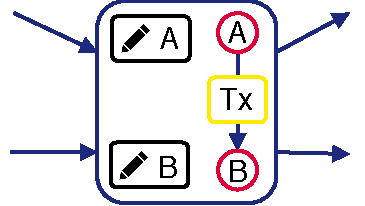
\includegraphics[width=.7\linewidth]{xchange/assets/trustchain_tutorial_3}
		\caption{To increase security, each block also references the previous block in the chain of a record counterparty.}
		\label{fig:trustchain_tutorial_3}
	\end{subfigure}
	\begin{subfigure}[t]{.45\textwidth}
		\centering
		\captionsetup{width=.9\linewidth}
		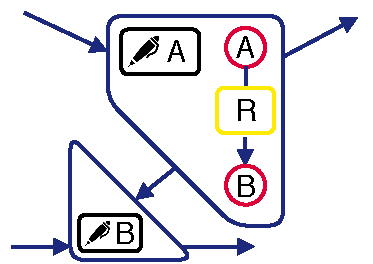
\includegraphics[width=.71\linewidth]{xchange/assets/trustchain_tutorial_4}
		\caption{To improve scalability, we extend the TrustChain structure to support concurrent block creation.}
		\label{fig:trustchain_tutorial_4}
	\end{subfigure}\hspace{0.05\textwidth}%
	\caption{Storing records in TrustChain.}
	\label{fig:trustchain_tutorial}
\end{figure*}

We argue that TrustChain is a suitable ledger to store \ModelName{} records, for the following four reasons.
First, TrustChain allows participants to verify the integrity of other individual ledgers themselves, and determine whether a party is already involved in a trade or not.
There is no requirement to reach a global consensus on the integrity of included records.
Second, TrustChain does not require network-wide replication of all records but enables individuals to selectively share parts of their individual ledger with others.
This feature reduces storage requirements and allows \ModelName{} to also run on devices with storage limitations, as we demonstrate in Section~\ref{sec:exp_trading_low_devices}.
Third, the TrustChain structure is optimized to store bilateral records that are signed by two parties.
This aligns well with the \ModelName{} trading protocol since many operations could benefit from support for bilateral records (for example, trade agreements).
Finally, TrustChain is already being used by various decentralized applications that require accounting features, such as self-sovereign identities and inter-bank payments~\cite{stokkink2018deployment,de2018real}.
At the time of writing, the public TrustChain ledger contains over 160 million records, created by 96'000 unique identities.\footnote{See \url{http://explorer.tribler.org}}

\subsection{Storing TrustChain Records}
We now outline how a record between two interacting users $ A $ and $ B $ is recorded in TrustChain, see Figure \ref{fig:trustchain_tutorial}.
Each record is stored within a block.
Figure \ref{fig:trustchain_tutorial_1} highlights one block containing a record between $ A $ and $ B $.
Each block contains a single record (\emph{R}).
A record can be a generic description of any interaction between users, for instance, a trade agreement or a payment.
Both interacting parties digitally sign the block with the record by using any secure digital signing algorithm.
These signatures are included in the block and ensure that participation by both parties is irrefutable.
It also confirms that both parties agree with the record itself.
Others can effectively verify the digital signatures included in a block.
After all required signatures have been added to a block, the block is committed to the local databases of the two interacting parties and broadcast to a limited number of random peers in the network.

The security of stored blocks is improved by linking them together, incrementally ordered by creation time.
In particular, each block is extended with a description (hash) of the previous block.
Each block has a sequence number that indicates its position in the individual ledger.
This results in the structure shown in Figure \ref{fig:trustchain_tutorial_2}.
As a result, each user maintains their individual ledger, which contains all records in which they have participated.
This sets TrustChain apart from the structure of traditional blockchains, where the entire network maintains a single, linear ledger.

Note how the blockchain structure in Figure \ref{fig:trustchain_tutorial_2} allows $ A $ to modify blocks in their individual ledger without being detected by others.
In particular, $ A $ can reorder the blocks in its individual ledger since validity can quickly be restored by recomputing all hashes.
In most blockchain applications, the global consensus mechanism prevents this kind of manipulation.
TrustChain uses a more efficient approach: each block is extended with an additional (hash) pointer that points to the previous block in the individual ledger of the counterparty.
This is visualized in Figure \ref{fig:trustchain_tutorial_3}.
Each block now has exactly two incoming and two outgoing (hash) pointers, except for the last block in an individual ledger, which only has two incoming pointers.
Modifications of the individual ledger by $ A $, like reordering or removing blocks, can now be detected by one or more counterparties.
To prove this fraud, a counterparty reveals both the correct block and the invalid block created by $ A $.

When two parties transact and create a block, their chains essentially become entangled.
When users create more records with others, it leads to the directed acyclic graph (DAG) structure, as shown in Figure \ref{fig:trustchain}.
Figure \ref{fig:trustchain} shows seven blocks, created by seven unique users.
Each block is added once to the individual ledger of all parties involved in the record.
For a more advanced analysis of the technical specifications and security of TrustChain, we refer the reader to the original paper by Otte et al.~\cite{otte2017trustchain}.

\begin{figure}[t]
	\centering
	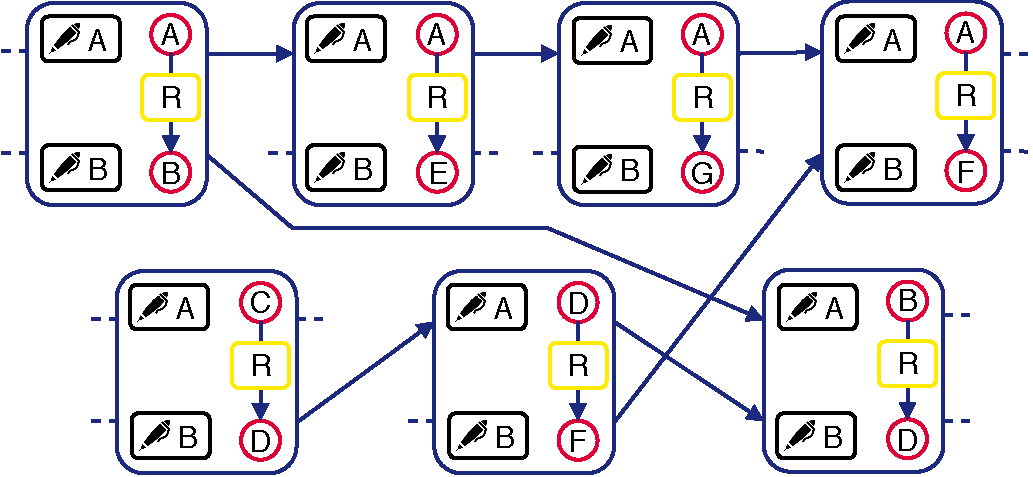
\includegraphics[width=.8\linewidth]{xchange/assets/trustchain}
	\caption{The TrustChain ledger, with seven blocks created by seven participants.}
	\label{fig:trustchain}
\end{figure}

\subsection{Improving TrustChain Scalability}
According to Otte et al., TrustChain is designed to scale~\cite{otte2017trustchain}.
However, we identify that its design limits a user to one pending block creation at once.
The main issue is that the digital signature of a counterparty is required before a new block can be appended to an individual ledger (since the input for the hash of each new block includes all signatures in the previous block).
This enables an attack where a malicious user can purposefully slow down the block creation of others by delaying the signing process of a bilateral transaction it is involved in.
It also limits the growth rate of individual ledgers and reduces the overall scalability of TrustChain.

We contribute to TrustChain and improve its scalability by adding support for \emph{concurrent block creation}.
The idea is to remove the requirement for a digital signature of the counterparty when appending new blocks to an individual ledger.
We believe that this concurrency is necessary since it allows traders to append new records without reliance on other parties.

Our solution is visualized in Figure \ref{fig:trustchain_tutorial_4}.
It shows a record between users $ A $ and $ B $, initiated by $ A $.
We partition a block in two parts, and each block partition is appended to the individual ledger of exactly one party.
Construction of a block between $ A $ and $ B $ now proceeds as follows: first, user $ A $ creates a record by constructing a block partition with the record content and its digital signature.
User $ A $ adds this block partition to its individual ledger immediately (note that it does not include the digital signature of $ B $).
$ A $ now sends the block partition to $ B $.
If $ B $ agrees with the transaction, it signs the block partition created by $ A $, adds it to its individual ledger, and sends his block partition (with their signature) back to $ A $.
User $ A $ stores the block partition created by $ B $ in its local database.
The participation of both parties in this record can now be proven with both block partitions.
This mechanism allows users to be involved in multiple block constructions at once.

\begin{figure}[t]
	\centering
	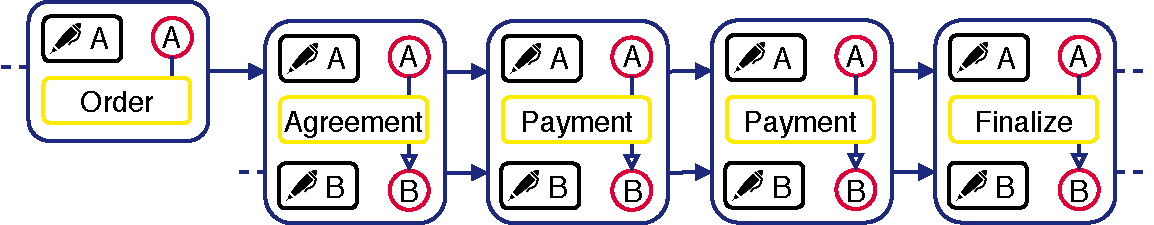
\includegraphics[width=\linewidth]{xchange/assets/trustchain_market}
	\caption{A part of the TrustChain ledger, storing an order created by a maker $ A $, and full specifications of a finished trade between $ A $ and $ B $.}
	\label{fig:trustchain_market}
\end{figure}

\subsection{Logging Trade Records on TrustChain}
We now outline how \texttt{Order}, \texttt{CancelOrder}, \texttt{Agreement}, \texttt{Payment}, \texttt{Finalize} and \texttt{CancelTrade} records are stored on TrustChain.
Figure \ref{fig:trustchain_market} shows a part of the TrustChain ledgers of traders $ A $ and $ B $.
It includes a sequence of records that indicate a finished trade between $ A $ and $ B $.
Trade agreements, created during the second phase in the \ModelName{} protocol, are stored within a bilateral \texttt{Agreement} record and digitally signed by both involved traders.
Individual payments are stored within bilateral \texttt{Payment} records.
A \texttt{Payment} record signed by both parties indicates that the payer has conducted the payment and that the payee has observed the payment.
Finally, a trade finalization is stored within a bilateral \texttt{Finalize} record.
Since the overhead of creating new TrustChain records is low, we also store orders as unilateral \texttt{Order} records in individual ledgers.
A unilateral record only contains the digital signature of its creator.
Figure~\ref{fig:trustchain_market} shows a \texttt{Order} record, created by maker $ A $.
Furthermore, \texttt{CancelOrder} and \texttt{CancelTrade} records are also included as unilateral records in one's individual TrustChain ledger.

A particular issue is that the fragmented nature of the TrustChain DAG makes it difficult for takers to discover interesting orders quickly.
Specifically, \texttt{Order} records are by default only stored in the individual ledger of the order creator.
Therefore, we introduce \emph{matchmakers}, peers that continuously collect the TrustChain records of other peers in the network, and organize the information in \texttt{Order} records in a local database.
Matchmakers aggregate orders, and takers can query the database of matchmakers to find interesting orders.
Makers also send their TrustChain blocks with an \texttt{Order} record to known matchmakers after creation.
The role of matchmakers in \ModelName{} is comparable with that of relay nodes in 0x~\cite{warren20170x} and indexers in AirSwap~\cite{airswap}.

\section{Implementation and Evaluation}
\label{sec:evaluation}
In this section we present the implementation of \ModelName{} and our experimental evaluation.
The evaluation answers the following three questions: (1) how effective is \ModelName{} at reducing fraud gains? (2) what is the overhead of \ModelName{}, in terms of trade duration, when \ModelName{} is deployed on low-resource devices? And (3) How scalable is \ModelName{} in terms of throughput and trade duration when increasing the system load?

The following experiments quantify the effectiveness, performance and overhead of our \ModelName{} mechanism.
During these experiments, we assume that asset settlement is instant.
As such, we do not actually connect a permissioned ledger to \ModelName{} for asset transfers.
We believe this is a reasonable experiment setup since our aim is to evaluate the scalability and overhead of our approach without the interference of external systems.

\subsection{Implementation Details}
\label{sec:implementation}
We have implemented the \ModelName{} in the Python 3 programming language.
Our implementation spans a total of 4'702 lines of code and uses an event-based programming model, powered by the built-in \texttt{asyncio} library.
The implementation is open source and all software artifacts (source code, tests, and documentation) are published on GitHub.\footnote{See \url{https://github.com/tribler/anydex-core}}

\textbf{Networking.}
We have built \ModelName{} on top of an existing networking library that is also used by TrustChain.
%Since TrustChain is built upon the IPv8 decentralized networking library, we decided to adopt it for all network communication generated by \ModelName{}.
%Our motivation for this is that TrustChain utilizes the same networking library.
This library provides the functionality to devise decentralized overlay networks and has built-in support for authenticated network communication, custom message definitions, and UDP hole punching.\footnote{See \url{https://github.com/tribler/py-ipv8}}
For efficiency reasons, the UDP protocol is used for message exchange between peers.
%It requires no central server to run, except for bootstrapping in the live network.
%Our implementation of \ModelName{} defines 15 distinct types of network messages, of which 11 are used to notify traders about matched orders and to manage execution of trade.

\textbf{Request Stores.}
To correctly process incoming messages during trade negotiation (phase II of the \ModelName{} protocol, see Section~\ref{sec:protocol}), \ModelName{} stores the state of outgoing messages.
The state of outgoing messages is stored in distinct \emph{request stores}.
For each outgoing message that has a state attached, a unique identifier is generated, a new request store containing this identifier is created and the generated identifier is appended to the outgoing message.
Traders that receive a message with this identifier are required to include the same identifier in their response message.
Incoming response messages with an unknown identifier are discarded and not processed further.
Each request store can have an optional timeout, indicating the duration after which the request store times out.
When a request store times out, it is deleted.

\textbf{Wallets.}
\ModelName{} organizes different types of assets within wallets.
These wallets provide a convenient interface to the information provided by connected blockchain platforms.
Wallets expose functionality to query the existence of specific transactions, fetch the content of specific transactions, and to transfer available assets to another trader.

Our implementation contains a \texttt{Wallet} base class that can be extended by programmers to create wallets that store different types of assets.
For testing purposes, we have implemented a \texttt{DummyWallet}, which is used when executing the unit tests and when running the experiments described in this section.
This wallet does not interact with any blockchain and simply waits for some duration before returning a (fake) response.

\begin{figure}
	\centering
	\begin{subfigure}{.9\textwidth}
		\centering
		\captionsetup{width=.9\linewidth}
		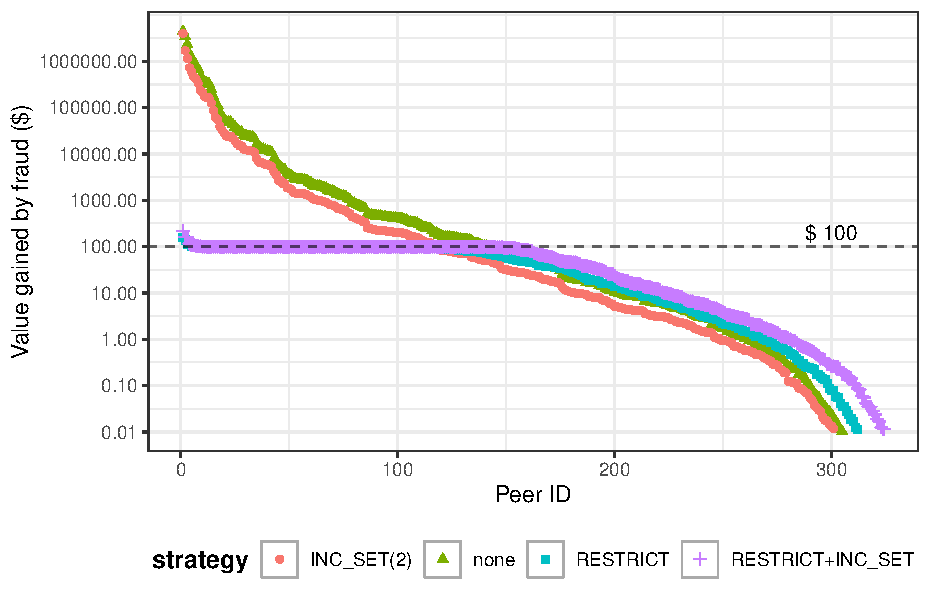
\includegraphics[width=.95\linewidth]{xchange/assets/experiments/fraud/gained_per_user}
		\caption{The economic gains of adversaries}
		\label{fig:fraud_experiment_gained}
	\end{subfigure}\vspace{0.3cm}
	\begin{subfigure}{.9\textwidth}
		\centering
		\captionsetup{width=.9\linewidth}
		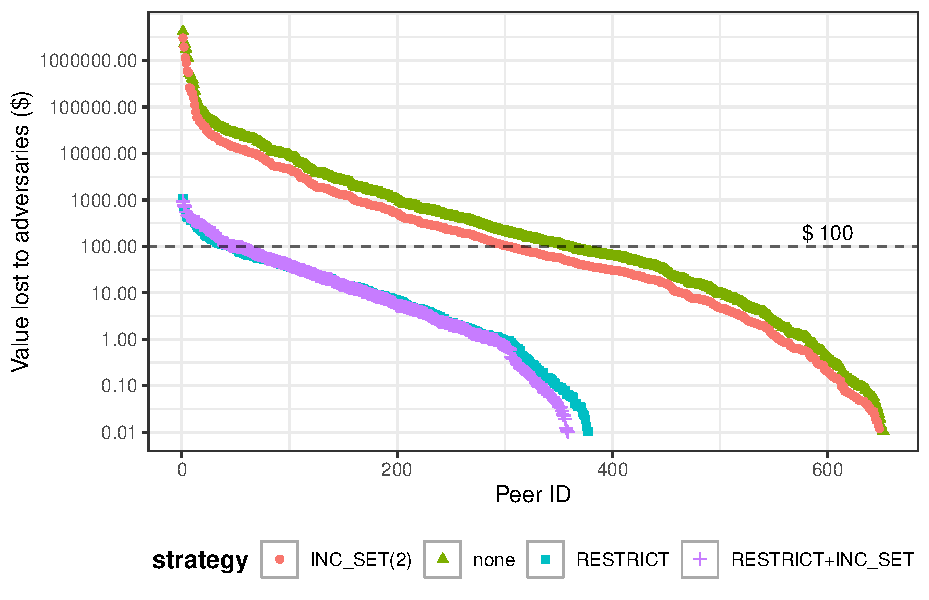
\includegraphics[width=.95\linewidth]{xchange/assets/experiments/fraud/losses_per_user}
		\caption{The economic losses of traders}
		\label{fig:fraud_experiment_losses}
	\end{subfigure}%
	\caption{The economic gains of adversaries and the losses of traders when replaying 230'000 BitShares orders with \ModelName{}, for different risk mitigation strategies. We have fixed the trust threshold $ U $ to \$100.}
	\label{fig:fraud_experiments}
\end{figure}

\subsection{Reducing Fraud Gains}
\label{sec:xchange_fraud_experiment}
Our first experiment quantifies the effectiveness of reducing fraud gains when trading with \ModelName{}.
We experimentally show the effectiveness of the risk mitigation strategies discussed in Section~\ref{sec:limit_risk}.

\textbf{Setup and Workload.}
For this experiment, we reconstruct a real-world dataset, containing buy and sell orders published on the BitShares blockchain~\cite{schuh2015bitshares}.
The BitShares platform enables users to issue custom assets and to trade these assets with others.
We extract the buy and sell orders made during the last week at the moment of writing, and replay them with \ModelName{}.
This results in a dataset with 230'000 orders, consisting of 125'527 buy orders, 104'423 sell orders and 212'489 cancellation events of existing orders.
These orders have been created by 1'161 unique users and involve 243 different assets.
Our data includes the orders created between November 11, 2020, and November 18, 2020.
Since our dataset does not contain granular temporal information on order creation and cancellation, we assume that each order is uniformly created in the time interval between the last block and the block that contains this specific event.
To accurately apply the \emph{bounded obligations} strategy (see Section~\ref{sec:bounded_obligations}), we compile a list with the market price of all assets in our dataset, expressed in USD, by crawling a major BitShares block explorer.\footnote{See \url{https://cryptofresh.com/api/docs}}
We were unable to accurately determine the market price for 36 assets since they have a low or zero trading volume.
We ignore the orders trading such assets during our experiment.
We have published all scripts to construct this dataset in a separate GitHub repository.\footnote{See \url{https://github.com/devos50/bitshares-orderbook-scripts}}

Since it is impractical to replay all the events in our dataset in real-time, we substitute our networking library with a custom discrete event simulator that is fully compatible with the \texttt{asyncio} library.
At the start of the experiment, we create wallets for all peers with an unlimited amount of assets.
To test the limitations of our mechanism in a highly adversarial setting, we model all peers as fraudsters, where they steal incoming assets whenever possible.
Specifically, they commit counterparty fraud by not issuing a subsequent asset transfer after receiving some assets.
During our experiment, a single peer acts as matchmaker and notifies traders about opportunities for their buy and sell orders.
We fix the trust threshold $ U $ to \$100 for all peers when the \emph{bounded obligations} strategy is enabled, meaning that the economic gains of an adversary are at most \$100.

We test the effectiveness of our mechanism with combinations of the two risk mitigation strategies discussed in Section~\ref{sec:limit_risk}.
With the \texttt{INC\_SET(k)} strategy, we refer to the incremental settlement strategy where each trader makes $ k $ payments to the counterparty during a single trade.
The \texttt{RESTRICT} strategy denotes the strategy where a trader follows the \emph{bounded obligations} strategy to verify whether it should trade with another party or not (see Section \ref{sec:limit_risk}).
We consider four experiment settings in total, with combinations of the \texttt{RESTRICT} and \texttt{INC\_SET} strategies, and when no risk mitigation strategy is active.
We note that the number of incremental payments when enabling the \texttt{RESTRICT} strategy is not fixed and depends on the current and prospective obligations of a counterparty.

\textbf{Results.}
We show the results of our fraud experiments in Figure~\ref{fig:fraud_experiments}.
Figure~\ref{fig:fraud_experiment_gained} shows the economic gains of adversaries, for combinations of the risk mitigation strategies discussed in Section~\ref{sec:limit_risk}.
We show the value gained by adversaries on a logarithmic vertical axis.
During our experiment we keep track of the fraud committed by adversaries, and sort these peers by the amount of fraud they have committed in USD.
The horizontal axis shows the identifier of these peers.
The total fraud gain without any risk mitigation strategy is \$18.5 million.
This number is reduced to just \$18'609 under the \texttt{RESTRICT+INC\_SET} strategy, \emph{a reduction of 99.9\%}.
Under the \texttt{RESTRICT} strategy, the total fraud gain is \$16'260, lower than the gains under the \texttt{RESTRICT+INC\_SET} strategy.
We address this due to the fact that some trade proposals are being denied since they cannot be completed without incremental settlement; these trades, however, might have been possible when using incremental settlement, which would have resulted in more fraud instances.
We also note that a few adversaries have committed fraud with a total value of over \$1 million when running without any risk mitigation strategy, and under the \texttt{INC\_SET(2)} strategy.
These successful adversaries likely created orders with competitive market prices, resulting in more trade proposals and opportunity for fraud.

Figure~14a clearly shows the effectiveness of the \emph{bounded obligations} strategy.
However, we observe that a few adversaries were able to commit fraud with a total value that exceeds our bound of \$100.
For the \texttt{RESTRICT+INC\_SET} strategy, twelve adversaries have committed fraud with a total value over \$100.
We have identified that this issue arises from the weak consistency guarantees by TrustChain.
Specifically, a trader $ A $ can be involved in the negotiation about many other orders at the same time, which together would exceed the bound of \$100.
When all counterparties query the individual ledger of $ A $ around the same time, all these parties might decide that it is safe to trade with $ A $ and as a result engage in trade with $ A $.
In addition, a counterparty might deliberately refrain from send its latest record(s) back, which we refer to as the \emph{record withholding attack}.
To address these issues, we suggest two extensions to \ModelName{} and TrustChain.
First, \ModelName{} can also record all the trade proposals, and their responses by counterparties (accept or reject).
Counterparties can take the outstanding trade proposals into consideration when applying risk mitigation.
To address the record withholding attack, a party can disseminate the latest record of its counterparty in Distributed Hash Table (DHT), e.g., Kademlia~\cite{maymounkov2002kademlia}.
Traders can then query the DHT network to fetch the latest record of a party $ A $, and then query the individual ledger of $ A $ up to that record.
Even with this timing issue present, Figure~14a still shows that our risk mitigation is highly effective and is capable of significantly reducing fraud gains.

Figure~\ref{fig:fraud_experiment_losses} shows the economic losses of traders, for different risk mitigation strategies.
Again, we notice that the \emph{bounded obligations} strategy significantly reduces the economic losses of traders.
The maximum individual loss when applying no risk mitigation strategy and under the \texttt{RESTRICT+INC\_SET} strategy is \$4'255'731 and \$928.79, respectively.
Figure~\ref{fig:fraud_experiment_losses} also highlights the effectiveness of incremental settlement under the \texttt{INC\_SET(2)} strategy, compared to when no risk mitigation strategy is applied.
In comparison to the fraud gains by adversaries, the economic losses by individual traders are not bounded but they are manageable.

\textbf{Conclusion.}
Our experiment with real-world data proves that the risk mitigation strategies by \ModelName{} are effective and significantly reduce fraud gains of adversaries.
In particular, we have experimentally proven that incremental settlement indeed decreases fraud losses, and that bounded obligations bounds the economic gains by adversaries.

\subsection{Trading on Low-resource Devices}
\label{sec:exp_trading_low_devices}
Our second experiment quantifies the latency added by \ModelName{} when conducting a trade between two low-resource devices.

\textbf{Setup and Workload.}
This experiment is conducted with two hosted Raspberry Pis (3rd generation, model B+).
The devices run the Raspbian Stretch operating system and the Python 3.5 interpreter.
One device assumes the identity of trader $ A $, and the other device acts as trader $ B $.
Furthermore, one device creates a new order, and the other device fulfills the order.
The experiment is executed in an isolated environment: there is only network communication between the two Raspberry Pis.
For this experiment, we use two different subclasses of \texttt{DummyWallet}, representing different assets.
To measure the overhead of \ModelName{}, we configure these wallets such that assets instantly arrive when being transferred to another wallet.
During the experiment, we log the timestamp of several events.
At $ t=0 $, the maker creates a new order.
The trade is finished when both trading parties have signed a \texttt{Finalize} record and have committed this record to their individual ledgers.

\begin{figure}[t]
	\centering
	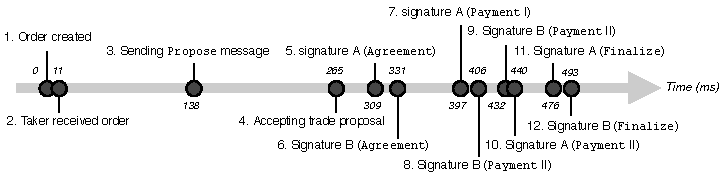
\includegraphics[width=\linewidth]{xchange/assets/trade_timeline}
	\caption{A timeline of the events during a single trade between a maker $ A $ and a taker $ B $. The experiment is conducted on two hosted Raspberry Pis (3rd generation, model B+). The total duration of the trade is 493 milliseconds.}
	\label{fig:trade_timeline}
\end{figure}

\textbf{Results.}
Figure \ref{fig:trade_timeline} shows a timeline of the events during a single trade between the two Raspberry Pis.
The full trade sequence, from the moment of order creation to mutual possession of a dual-signed \texttt{Finalize} transaction, completes in 493 milliseconds, less than half a second.
Almost half of the trade duration, 254 milliseconds, is spent in phase II of the \ModelName{} trading protocol, the trade negotiation phase.
During this phase, a trader determines whether a counterparty is already involved in a trade by inspection of the records in the TrustChain ledger of the other party.

\textbf{Conclusion.}
This experiment shows that a full trade, including order creation, can be completed within half a second on low-resource devices if asset transfer would be instant.
Based on this experiment, we argue that the deployment of \ModelName{} in an Internet-of-Things (IoT) environment would be viable since its communication and transaction creation overhead is minimal.
Asset management is a common feature in IoT~\cite{gilchrist2016industry}.
\ModelName{} can be used to coordinate asset exchange between different IoT environments.
However, our trading protocol requires periodic inspection of blockchain during an ongoing trade.
Since maintaining a full transaction history is not realistic given the storage restrictions of IoT devices, \ModelName{} should rely on dedicated full nodes that have to appropriate credentials to participate in a specific blockchain.
We believe that devices with less processing capabilities than Raspberry Pis are still capable of maintaining and securing TrustChain records.
This belief should be verified with further experimentation through a small-scale deployment of \ModelName{} in an IoT environment where blockchain-based assets are managed and traded.

Even though the low trade duration on low-resource devices is a promising result, the experiment is not representative of a realistic trading environment where there are many traders creating orders and exchanging assets simultaneously.
Furthermore, the prior experiment does not reveal the impact of our risk mitigation strategies on performance.
Therefore, our next experiment focuses on the scalability of \ModelName{} and shows how our mechanism behaves under a higher system load.

\subsection{Scalability of \ModelName{}}
\label{subsec:scalability_experiment}
We now perform scalability experiments to quantify the performance of \ModelName{} as the system load and network size increases.

\textbf{Setup and Workload.}
To explore the limitations and overhead of \ModelName{}, we conduct scalability experiments on our university cluster.
The detailed specifications of the hardware and runtime environment can be found online.\footnote{See \url{https://www.cs.vu.nl/das5/}}
Our infrastructure allows us to reserve computing nodes and deploy instances of \ModelName{} on each node.
We use the Gumby experiment framework to orchestrate the deployment of \ModelName{} instances onto computing nodes and to extract results from experiment artifacts.\footnote{See \url{https://github.com/tribler/gumby}}
The scalability experiment is controlled by a \emph{scenario file}, a chronologically ordered list of actions which are executed by all or by a subset of running instances, at specific points in time after the experiment starts.
Each run is performed at least five times, and the results are averaged.

We increase the system load, namely the number of new orders being created every second.
As the system load grows, so does the number of traders in the network.
We devise a synthetic dataset to determine the performance of \ModelName{} under a predictable arrival rate of orders.
In a network with $ n $ peers running \ModelName{}, $ n $ orders are created every half a second.
To avoid the situation where all instances create new orders at the same time, the starting time of this periodic order creation is uniformly distributed over all peers, based on their assigned IDs (ranging from 1 to $ n $).
Each peer acts as a matchmaker and sends a new order to four matchmakers, which each peer randomly selects when the experiment starts.
The experiment lasts for 30 seconds, after which $ 30n $ orders are created in total.
Each order buys a single token in return for another token, to make matchmaking a predictable process.
After 30 seconds, the experiment is terminated.

Scalability is measured as follows:
first, we analyse the peak \emph{throughput} observed during the experiment, in terms of trades per second.
Second, we consider the average order fulfil \emph{latency}, which is the time between the creation of an order and the time until this order has been completed (the order creator has exchanged all assets as specified in the order).

\begin{figure}[t]
	\centering
	\begin{subfigure}{.9\textwidth}
		\centering
		\captionsetup{width=.9\linewidth}
		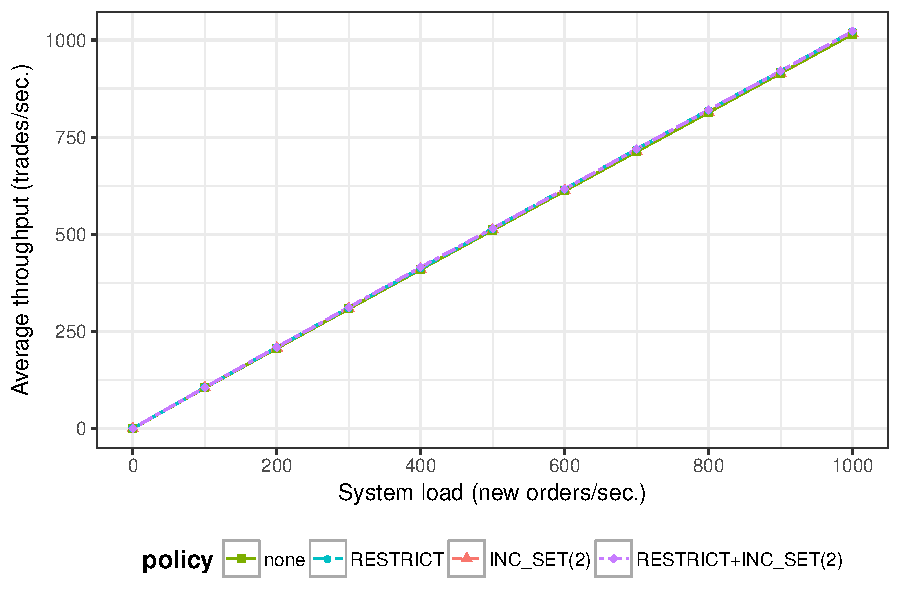
\includegraphics[width=.95\linewidth]{xchange/assets/experiments/scalability}
		\caption{Peak throughput}
		\label{fig:scalability}
	\end{subfigure}\vspace{0.3cm}
	\begin{subfigure}{.9\textwidth}
		\centering
		\captionsetup{width=.9\linewidth}
		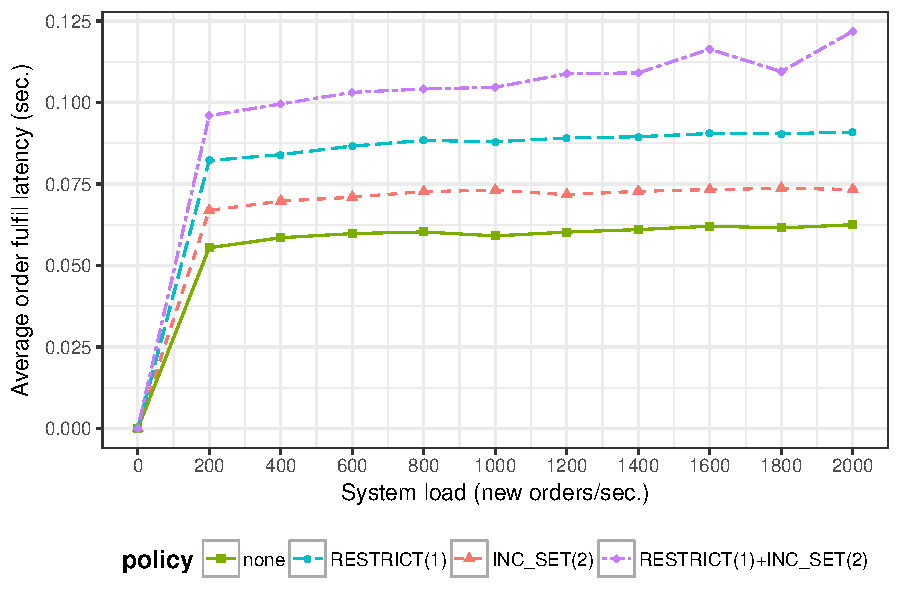
\includegraphics[width=.95\linewidth]{xchange/assets/experiments/latency}
		\caption{Average order fulfil latency}
		\label{fig:latency}
	\end{subfigure}%
	\caption{The peak throughput and order fulfil latencies as the system load increases.}
	\label{fig:scalability_latency}
\end{figure}

\textbf{Results.}
The results of the scalability experiments are presented in Figure~\ref{fig:scalability_latency}.
We run each experiment with a specific system load up to 1.000 deployed instances (which is close to the limitations of the used hardware).
Figure~\ref{fig:scalability} shows how the peak throughput (expressed in trades per second, vertical axis) behaves with respect to the system load (horizontal axis).
All experiment settings hint at linear scalability as the system load increases.
Furthermore, enabling risk mitigation strategies does not appear to have a notable effect on the peak throughput.
Experimentation on more compute nodes should reveal whether this trend continues when the system load exceeds 1.000 new orders per second.

Figure~\ref{fig:latency} shows the average order fulfil latency when the system load increases, for the four risk mitigation strategies.
The average order fulfil latency remains largely constant when the system load grows.
Applying the restriction and incremental settlement strategies increases the average order fulfil latency, since more operations have to be performed to successfully complete an order.
We observe a moderate increase of latency when applying the \texttt{RESTRICT+INC\_SET} strategies when the system load grows to 1.000 trades per second.
The high system load is likely to increase the duration of individual trades beyond 0.5 seconds, which means that the \texttt{RESTRICT} strategy prevents traders from initiating a new trade with others.
Since a trader now has to find a new party to trade with, the average order fulfil latency increases.

\textbf{Conclusion.}
The main finding of this experiment is that the throughput (trades per second) scales linearly with respect to the system load and network size.
We also observe that the average order fulfil latency remains largely constant as the system load grows.
Further experimentation should reveal whether these trends continue with an even higher system load.

\section{Conclusions}
We have presented \ModelName{}, a universal mechanism for asset exchange between permissioned blockchain.
\ModelName{} facilitates asset exchange without relying on particular transaction types or trusted third parties to mediate in the trading process.
\ModelName{} records the initiation of a trade, individual payments, and the completion of a trade in a distributed log.
By devising a set of rules that define when a party should engage in a new trade, we have limited the economic gains of adversarial parties.
Specifically, when an adversary commits counterparty fraud, any further trade with this adversary are refused by honest parties until the fraud is resolved.
Incremental settlement further reduces economic gains by splitting each payment into multiple, smaller ones.

We have implemented \ModelName{} and open-sourced its implementation.
By replaying a dataset containing orders published on the BitShares blockchain, we have showed that \ModelName{} can significantly reduce fraud gains.
We have also demonstrated the viability of trading on devices with low hardware capabilities.
A single trade can be completed within half a second if asset transfers on external blockchain platforms would finish instantly.
With a scalability experiment on our compute cluster, we achieved over 1'000 trades per second and found that the throughput of \ModelName{} in terms of trades per second scales linearly with the system load and network size.

We end by highlighting two promising research directions for further work.
First, it would be helpful to extend our mechanism with privacy-enhancing features that do not reveal full trade details to the network.
Second, our mechanism would benefit from a more extensive risk model that allows a trader to further reason about other traders while judging their trade proposals.
This risk model can, for example, also take into consideration the \enquote{response time} of a counterparty and classify slower counterparties as riskier.